%% =============================================================================
%% Projeto Base - Artigo de TCC com abnTeX2
%% Customizado para a UNIJUÍ
%% Template desenvolvido e mantido por: Prof. Eldair F. Dornelles
%% A versão mais atualizada deste template pode ser obtida no GitHub:
%% https://github.com/dornelles/tcc-artigo-template-latex
%% Qualquer sugestão de melhoria será bem vinda, 
%% Contato pelo e-mail: eldair.dornelles@unijui.edu.br
%% =============================================================================

\documentclass[
    12pt,               % tamanho da fonte
    oneside,            % para impressão frente e verso (use oneside para apenas frente)
    a4paper,            % tamanho do papel
    chapter=TITLE,      % títulos de capítulos em maiúsculas
    section=TITLE,      % títulos de seções em maiúsculas
    english,            % idioma adicional para hifenização
    brazil,             % o último idioma é o principal do documento
    article             % formatação como artigo
]{abntex2}

% ==============================================================================
% PACOTES ESSENCIAIS
% ==============================================================================

% --- Codificação e fontes ---
\usepackage[T1]{fontenc}        % seleção de códigos de fonte
\usepackage[utf8]{inputenc}     % codificação do documento (conversão automática dos acentos)
% \usepackage{lmodern}          % comentado: a fonte agora está definida no arquivo unijui.sty

% --- Pacotes de citações ---
\usepackage[brazilian,hyperpageref]{backref}  % páginas com as citações na bibl
\usepackage[alf,bibjustif]{abntex2cite}        % citações padrão ABNT (bibjustif = referências justificadas)

% --- Pacotes matemáticos ---
\usepackage{amsmath}
\usepackage{amssymb}

% --- Pacotes gráficos ---
\usepackage{graphicx}           % inclusão de gráficos
% NOTA: NÃO usar \usepackage{float} com abnTeX2/memoir - conflita com \newfloat
\usepackage{subfig}             % subfiguras
\usepackage{pdfpages}           % inclusão de páginas PDF

% --- Pacotes de tabelas ---
\usepackage{booktabs}           % tabelas profissionais
\usepackage{multirow}           % células que ocupam várias linhas
\usepackage{longtable}          % tabelas longas (múltiplas páginas)
\usepackage{array}              % personalização de colunas

% --- Outros pacotes úteis ---
\usepackage{microtype}          % melhorias de justificação
\usepackage{indentfirst}        % indenta o primeiro parágrafo de cada seção
\usepackage{color}              % controle de cores
\usepackage{xcolor}             % cores avançadas
\usepackage{listings}           % listagens de código-fonte
\usepackage{enumitem}           % listas personalizadas
\usepackage{lipsum}             % geração de texto fictício (remover na versão final)
\usepackage{totcount}           % conta o total de floats (figuras, tabelas, etc.) no documento

% --- Customizações UNIJUÍ ---
\input{unijui.sty}

% ==============================================================================
% CONFIGURAÇÕES DO PACOTE BACKREF
% ==============================================================================
% Configurações do pacote backref
% Usado sem a opção hyperpageref de backref
\renewcommand{\backrefpagesname}{Citado na(s) página(s):~}
% Texto padrão antes do número das páginas
\renewcommand{\backref}{}
% Define os textos da citação
\renewcommand*{\backrefalt}[4]{
    \ifcase #1 %
        Nenhuma citação no texto.%
    \or
        Citado na página #2.%
    \else
        Citado #1 vezes nas páginas #2.%
    \fi}%

% ==============================================================================
% CONFIGURAÇÕES DE LISTAGENS DE CÓDIGO
% ==============================================================================
\lstset{
    basicstyle=\ttfamily\small,
    numbers=left,
    numberstyle=\tiny\color{gray},
    stepnumber=1,
    numbersep=8pt,
    backgroundcolor=\color{white},
    showspaces=false,
    showstringspaces=false,
    showtabs=false,
    frame=single,
    rulecolor=\color{black},
    tabsize=2,
    captionpos=b,
    breaklines=true,
    breakatwhitespace=false,
    keywordstyle=\color{blue}\bfseries,
    commentstyle=\color{green!60!black},
    stringstyle=\color{red},
    escapeinside={\%*}{*)},
    literate=
        {á}{{\'a}}1 {é}{{\'e}}1 {í}{{\'i}}1 {ó}{{\'o}}1 {ú}{{\'u}}1
        {Á}{{\'A}}1 {É}{{\'E}}1 {Í}{{\'I}}1 {Ó}{{\'O}}1 {Ú}{{\'U}}1
        {ã}{{\~a}}1 {õ}{{\~o}}1 {Ã}{{\~A}}1 {Õ}{{\~O}}1
        {ç}{{\c{c}}}1 {Ç}{{\c{C}}}1
        {ê}{{\^e}}1 {â}{{\^a}}1 {ô}{{\^o}}1
}

% ==============================================================================
% DADOS DO TRABALHO
% ==============================================================================

% --- Informações do documento (preencher conforme o trabalho) ---

\titulo{DEPLOYDOCK: ARQUITETURA, IMPLEMENTAÇÃO E AVALIAÇÃO EMPÍRICA DE UMA PLATAFORMA COMO SERVIÇO (PaaS) AUTOHOSPEDADA COM FOCO EM HARDENING DE CONTÊINERES E GITOPS}
% \subtitulo{Subtítulo (se houver)}

\tituloemingles{DEPLOYDOCK: ARCHITECTURE, IMPLEMENTATION AND EMPIRICAL EVALUATION OF A SELF-HOSTED PLATFORM AS A SERVICE (PAAS) FOCUSED ON CONTAINER HARDENING AND GITOPS}
% \subtituloemingles{Subtitle (if any)}

\autor{Jean Kronbauer de Moura}
\local{Ijuí/RS}
\data{2026}
\orientador{Prof. Marcos Ronaldo Melo Cavalheiro}
\instituicao{%
    Universidade Regional do Noroeste do\\[1mm]
    Estado do Rio Grande do Sul
}

% -- Autores para o artigo --
\autoresartigo{
    Jean Kronbauer de Moura
    \thanks{Estudante do Curso de Ciência da Computação -- UNIJUÍ, Ijuí-RS, Brasil. E-mail: \texttt{jean.moura@sou.unijui.edu.br}} 
    \and 
    Marcos Ronaldo Melo Cavalheiro
    \thanks{Professor Orientador -- UNIJUÍ, Ijuí-RS, Brasil. E-mail: \texttt{marcos.cavalheiro@unijui.edu.br}}
}

% --- Informações específicas da UNIJUÍ (definidas no unijui.sty) ---
\campus{Ijuí}
\curso{Ciência da Computação}
\professordabanca{Prof. Marcos Ronaldo Melo Cavalheiro}
\datadabanca{03}{Nov}{2026}

% --- Preâmbulo (texto da folha de rosto e aprovação) ---
\preambulo{Trabalho de Conclusão de Curso apresentado ao Curso de Ciência da Computação da 
            Universidade Regional do Noroeste do Estado do Rio Grande do Sul - UNIJUÍ,
            como requisito parcial para a obtenção do título de Bacharel em Ciência da Computação}


% --- Texto de apresentação ---
\textoapresentacao{
    O presente Trabalho de Conclusão de Curso, intitulado \textbf{``DEPLOYDOCK: ARQUITETURA, IMPLEMENTAÇÃO E AVALIAÇÃO EMPÍRICA DE UMA PLATAFORMA COMO SERVIÇO (PaaS) AUTOHOSPEDADA COM FOCO EM HARDENING DE CONTÊINERES E GITOPS''}, é submetido ao Colegiado do Curso de Ciência da Computação da Universidade Regional do Noroeste do Estado do Rio Grande do Sul (UNIJUÍ) como requisito para a obtenção do grau de Bacharel em Ciência da Computação. O documento organiza-se no formato de Artigo Científico estruturado segundo as normas da ABNT e as diretrizes do manual institucional da universidade. \par
    A pesquisa investiga os desafios de sustentabilidade operacional, orquestração enxuta e segurança cibernética em infraestruturas autohospedadas, articulando a teoria de microsserviços e sistemas operacionais a um estudo empírico com baterias ponta a ponta e testes de estresse de hardware. Após as páginas pré-textuais, sucedem-se a Introdução, a Metodologia, o Referencial Teórico, o Desenvolvimento e Resultados, as Considerações Finais e os elementos pós-textuais (declaração de integridade no uso de ferramentas de IA, referências bibliográficas, apêndice e anexos comprobatórios).
}

% --- Resumo e Abstract ---
\resumoemportugues{%
A virtualização orientada a contêineres e a cultura DevOps revolucionaram o ciclo de desenvolvimento de software, tornando essencial a adoção de esteiras automatizadas de entrega contínua. Contudo, orquestradores como o Kubernetes apresentam elevada complexidade e sobrecarga computacional para servidores modestos e aplicações autohospedadas, enquanto plataformas PaaS de código aberto existentes frequentemente negligenciam proteções na camada de aplicação e o isolamento de privilégios em contêineres. Este trabalho apresenta o DeployDock, uma Plataforma como Serviço (PaaS) autohospedada, leve e orientada a GitOps desenvolvida em Python assíncrono (FastAPI), Docker SDK e proxy reverso Traefik v3. A solução incorpora um Web Application Firewall (WAF) ativo perimetral, cofre de variáveis de ambiente com criptografia Fernet (AES-128), ajuste dinâmico de quotas de CPU/RAM em tempo de execução sem interrupção de contêineres e rollback automatizado em falhas. Para validação experimental, construiu-se uma sonda autônoma independente submetendo a plataforma a 58 testes E2E, estresse multivariado de hardware e 11 testes transacionais no PostgreSQL 16. Os resultados comprovaram 100\% de aprovação funcional e bloqueio defensivo de ataques de SQLi, XSS, Path Traversal e RCE, score de hardening de 95/100 sob Linux corporativo e cumprimento rigoroso das propriedades ACID sob vazão superior a 3.200 inserções/s, operando sob uma pegada basal de memória de apenas 79,2 MB em repouso.
}
\palavraschaveemportugues{computação em nuvem; plataforma como serviço; docker; orquestração de contêineres; segurança da informação; gitops.}

\resumoemingles{
Container-based virtualization and DevOps practices have deeply transformed the software development lifecycle, making continuous delivery pipelines paramount. However, complex orchestrators such as Kubernetes impose excessive cognitive and resource overhead for small-to-medium servers and self-hosted deployments, whereas existing open-source PaaS alternatives often lack integrated application-layer firewalls and strict container privilege isolation. This study presents DeployDock, a lightweight, self-hosted, GitOps-oriented Platform as a Service (PaaS) built with asynchronous Python (FastAPI), the Docker SDK, and Traefik v3 reverse proxy. The platform embeds an active Web Application Firewall (WAF) middleware, secret storage encryption via Fernet (AES-128), live dynamic CPU/RAM cgroup quota tuning without container downtime, and instant automated rollback upon health check failures. For empirical validation, an independent autonomous probe evaluated DeployDock against 58 E2E assertions, heavy multi-core hardware stress benchmarks, and 11 transactional tests targeting PostgreSQL 16. Experimental findings demonstrated a 100\% pass rate across all functional suites, robust perimeter mitigation against SQLi, XSS, Path Traversal, and RCE vectors, a 95/100 container hardening score under enterprise Linux, and strict compliance with ACID guarantees under bulk insertion rates exceeding 3,200 rows/second, all while maintaining a remarkably low memory footprint of only 79.2 MB at idle.
}
\palavraschaveemingles{cloud computing; platform as a service; docker; container orchestration; information security; gitops.}




% ==============================================================================
% CONFIGURAÇÕES DE APARÊNCIA DO PDF FINAL
% ==============================================================================
\makeatletter
\hypersetup{
    pdftitle={\@title},
    pdfauthor={\@author},
    pdfsubject={\imprimirpreambulo},
    pdfcreator={LaTeX com abnTeX2},
    pdfkeywords={abnt}{latex}{abntex}{abntex2}{artigo}{tcc},
    colorlinks=true,        % false: links em caixas; true: links coloridos
    linkcolor=black,        % cor dos links internos
    citecolor=black,        % cor dos links para bibliografias
    filecolor=black,        % cor dos links de arquivos
    urlcolor=black,         % cor dos links de URLs
    bookmarksdepth=4
}
\makeatother

% ==============================================================================
% ESPAÇAMENTOS ENTRE LINHAS E PARÁGRAFOS
% ==============================================================================
% O tamanho do parágrafo é dado por:
\setlength{\parindent}{1.3cm}
% Controle do espaçamento entre um parágrafo e outro:
\setlength{\parskip}{0.2cm}  % tente também \onelineskip



% ==============================================================================
% INÍCIO DO DOCUMENTO
% ==============================================================================
\begin{document}

% Seleciona o idioma do documento
\selectlanguage{brazil}

% Retira espaço extra obsoleto entre as frases
\frenchspacing

% --- Imprimir página de créditos e marca d'água ---
% \imprimirpaginadecreditos
% \imprimirmarcadagua

% ==========================================================================
% ELEMENTOS PRÉ-TEXTUAIS
% ==========================================================================
\pretextual

% --- Capa ---
\imprimircapa

% --- Folha de rosto ---
% (o * indica que haverá a ficha bibliográfica)
\imprimirfolhaderosto

% --- Ficha catalográfica (inserir PDF gerado pela biblioteca) ---
% \begin{fichacatalografica}
%     \includepdf{fig_ficha_catalografica.pdf}
% \end{fichacatalografica}

% --- Folha da banca ---
\imprimirfolhadabanca

% --- Agradecimentos ---
\begin{agradecimentos}
    Agradeço primeiramente a Deus, pela dádiva da vida, saúde, força e clareza mental que me sustentaram ao longo de toda esta jornada acadêmica.

    Aos meus pais e familiares, pelo amor incondicional, apoio irrestrito, sacrifícios diários e por acreditarem no meu potencial em cada etapa desta caminhada. A compreensão e o incentivo de vocês foram essenciais para transformar este sonho em realidade.

    Ao meu orientador, Prof. Marcos Ronaldo Melo Cavalheiro, pela dedicação, confiança, valiosas orientações técnicas e acadêmicas, paciência e pelo compartilhamento generoso de conhecimento que nortearam o amadurecimento desta pesquisa.

    Aos professores do Curso de Ciência da Computação da Universidade Regional do Noroeste do Estado do Rio Grande do Sul (UNIJUÍ), que com zelo e excelência contribuíram para minha sólida formação profissional, despertando a paixão pela investigação científica e pela computação aplicada.

    Aos colegas de curso e amigos de jornada, pelos momentos de companheirismo, noites em claro resolvendo desafios de código, discussões enriquecedoras e pela amizade fraterna construída ao longo destes anos.

    Por fim, a toda a comunidade de software livre e de código aberto, cujo espírito de cooperação global disponibiliza ferramentas indispensáveis para a democratização e o progresso da tecnologia.
\end{agradecimentos}
\clearpage

% --- Epígrafe ---
\begin{epigrafe}
    \inserirepigrafe{Simplicity is prerequisite for reliability.}{Edsger W. Dijkstra}
\end{epigrafe}
\clearpage

% --- Lista de ilustrações (só aparece se houver figuras) ---
% Na primeira compilação os contadores podem ser 0; compile 2x para resultado correto.
\ifnum\totvalue{figcount}>0
    \pdfbookmark[0]{\listfigurename}{lof}
    \listoffigures*
    \clearpage
\fi

% --- Lista de quadros (só aparece se houver quadros) ---
\ifnum\totvalue{quacount}>0
    \pdfbookmark[0]{\listofquadrosname}{loq}
    \listofquadros*
    \clearpage
\fi

% --- Lista de tabelas (só aparece se houver tabelas) ---
\ifnum\totvalue{tabcount}>0
    \pdfbookmark[0]{\listtablename}{lot}
    \listoftables*
    \clearpage
\fi

% --- Lista de abreviaturas e siglas ---
\begin{siglas}
    \item[ACID] Atomicidade, Consistência, Isolamento e Durabilidade (\textit{Atomicity, Consistency, Isolation, Durability})
    \item[AES] Padrão Avançado de Criptografia (\textit{Advanced Encryption Standard})
    \item[API] Interface de Programação de Aplicações (\textit{Application Programming Interface})
    \item[ASGI] Interface de Gateway de Servidor Assíncrono (\textit{Asynchronous Server Gateway Interface})
    \item[CI/CD] Integração Contínua e Entrega Contínua (\textit{Continuous Integration / Continuous Delivery})
    \item[CPU] Unidade Central de Processamento (\textit{Central Processing Unit})
    \item[DoS] Negação de Serviço (\textit{Denial of Service})
    \item[DSR] Pesquisa em Ciência do Design (\textit{Design Science Research})
    \item[E2E] Ponta a Ponta (\textit{End-to-End})
    \item[HMAC] Código de Autenticação de Mensagens Baseado em Hash (\textit{Hash-based Message Authentication Code})
    \item[HTTP] Protocolo de Transferência de Hipertexto (\textit{Hypertext Transfer Protocol})
    \item[HTTPS] Protocolo de Transferência de Hipertexto Seguro (\textit{Hypertext Transfer Protocol Secure})
    \item[IOPS] Operações de Entrada/Saída por Segundo (\textit{Input/Output Operations Per Second})
    \item[JWT] Token Web JSON (\textit{JSON Web Token})
    \item[MFLOPS] Milhões de Operações de Ponto Flutuante por Segundo (\textit{Million Floating-Point Operations Per Second})
    \item[OSI] Interconexão de Sistemas Abertos (\textit{Open Systems Interconnection})
    \item[OWASP] Projeto Aberto de Segurança em Aplicações Web (\textit{Open Worldwide Application Security Project})
    \item[PaaS] Plataforma como Serviço (\textit{Platform as a Service})
    \item[PAT] Token de Acesso Pessoal (\textit{Personal Access Token})
    \item[PID] Identificador de Processo (\textit{Process Identifier})
    \item[RAM] Memória de Acesso Aleatório (\textit{Random Access Memory})
    \item[RBAC] Controle de Acesso Baseado em Papéis (\textit{Role-Based Access Control})
    \item[RCE] Execução Remota de Código (\textit{Remote Code Execution})
    \item[SGBDR] Sistema de Gerenciamento de Banco de Dados Relacional
    \item[SHA] Algoritmo de Hash Seguro (\textit{Secure Hash Algorithm})
    \item[SQL] Linguagem de Consulta Estruturada (\textit{Structured Query Language})
    \item[SQLi] Injeção de SQL (\textit{SQL Injection})
    \item[SSRF] Falsificação de Requisição do Lado do Servidor (\textit{Server-Side Request Forgery})
    \item[TLS] Segurança da Camada de Transporte (\textit{Transport Layer Security})
    \item[TOTP] Senha Descartável Baseada em Tempo (\textit{Time-Based One-Time Password})
    \item[TPS] Transações por Segundo (\textit{Transactions Per Second})
    \item[TTFB] Tempo até o Primeiro Byte (\textit{Time To First Byte})
    \item[WAF] Firewall de Aplicações Web (\textit{Web Application Firewall})
    \item[WAL] Log de Pré-Gravação (\textit{Write-Ahead Logging})
    \item[XSS] Scripting em Múltiplos Sites (\textit{Cross-Site Scripting})
\end{siglas}

% --- Sumário ---
\pdfbookmark[0]{\contentsname}{toc}
\tableofcontents*
\cleardoublepage


% --- Página de Apresentação ---
\begin{apresentacao}
    \imprimirapresentacao
\end{apresentacao}
\newpage

% --- Página de Resumo e Abstract ---
\imprimirpaginaresumos


% ==========================================================================
% ELEMENTOS TEXTUAIS
% ==========================================================================
\textual

% --- Inclusão dos capítulos ---
% ==============================================================================
% CAPÍTULO 1 - INTRODUÇÃO
% ==============================================================================

\section{Introdução}
\label{sec:introducao}

A consolidação da computação em nuvem e a transição de monólitos de software para arquiteturas baseadas em microsserviços transformaram radicalmente as etapas de desenvolvimento, teste e implantação de sistemas computacionais. No centro dessa transformação, a virtualização baseada em contêineres --- especialmente capitaneada pelo ecossistema Docker --- estabeleceu-se como padrão \textit{de facto} na indústria de software \cite{merkel2014}. Ao empacotar a aplicação com todas as suas dependências e bibliotecas em unidades atômicas e portáveis, os contêineres garantem previsibilidade e eliminam discrepâncias entre ambientes de homologação e produção \cite{combes2016}.

No entanto, o gerenciamento do ciclo de vida dessas aplicações conteinerizadas introduz uma camada substancial de complexidade operacional. Práticas modernas como a Entrega Contínua (\textit{Continuous Delivery}) \cite{humble2010} e o paradigma GitOps --- no qual repositórios de controle de versão atuam como a fonte única da verdade para o estado desejado da infraestrutura --- exigem esteiras automatizadas de construção (\textit{build}), provisionamento de certificados digitais, roteamento reverso de tráfego de rede e monitoramento de integridade (\textit{health check}).

Para atender a essas demandas, o mercado corporativo tradicionalmente recorre a orquestradores de contêineres em larga escala, dos quais o Kubernetes é o expoente mais difundido \cite{burns2016}. Embora o Kubernetes apresente capacidades sólidas de escalabilidade horizontal e resiliência em centros de dados distribuídos, sua adoção impõe uma sobrecarga computacional acentuada e uma curva de aprendizado íngreme. A complexidade de configuração baseada em centenas de manifestos YAML, o consumo excessivo de memória em repouso dos planos de controle (\textit{control plane}) e a necessidade de equipe especializada inviabilizam sua sustentabilidade econômica e técnica em infraestruturas modestas, pequenos servidores autohospedados (\textit{bare-metal} ou VPS), laboratórios acadêmicos e pequenas empresas de base tecnológica.

Como alternativa, consolidaram-se as Plataformas como Serviço (\textit{Platform as a Service} -- PaaS), tanto em ofertas proprietárias sob demanda na nuvem pública (tais como Heroku, Render e Railway), quanto em soluções de código aberto autohospedadas (\textit{self-hosted}), exemplificadas por CapRover, Dokploy e Coolify. Não obstante a evolução das ferramentas de código aberto, uma investigação aprofundada de suas arquiteturas revela lacunas críticas:
\begin{enumerate}[label=(\alph*)]
    \item \textbf{Vulnerabilidade na Camada de Aplicação:} a grande maioria dos orquestradores PaaS foca exclusivamente no roteamento HTTP (frequentemente via Traefik ou Nginx), transferindo integralmente a responsabilidade de mitigação de ataques à aplicação, carecendo de um Web Application Firewall (WAF) ativo e integrado capaz de neutralizar vetores como Injeção de SQL (\textit{SQL Injection}), \textit{Cross-Site Scripting} (XSS), \textit{Path Traversal} e Execução Remota de Código (RCE) antes que atinjam o núcleo do sistema;
    \item \textbf{Falta de Hardening Padrão no Contêiner:} por conveniência operacional, muitos contêineres gerenciados são criados sem imposição de restrições de privilégios (`no-new-privileges`), sem cotas estritas de criação de processos (`pids.max`), permitindo que falhas de código ou bibliotecas comprometidas provoquem esgotamento de recursos no hospedeiro (\textit{fork bomb}) ou escalação de privilégios via binários com bits SUID;
    \item \textbf{Gestão Rígida de Recursos:} o ajuste de quotas de memória RAM e núcleos de CPU geralmente demanda a interrupção completa e recriação do contêiner, interrompendo a prestação de serviços;
    \item \textbf{Ausência de Baterias de Auditoria Científica:} inexistem mecanismos integrados nas plataformas que permitam auditar e mensurar, de forma empírica e reprodutível, a conformidade de transações de bancos de dados relacionais com as propriedades ACID (Atomicidade, Consistência, Isolamento e Durabilidade) \cite{stonebraker1986}, bem como limites de estresse de CPU, memória, I/O e rede.
\end{enumerate}

Diante dessa problemática, emerge a seguinte questão de pesquisa: \textit{Como conceber, implementar e avaliar empiricamente uma Plataforma como Serviço (PaaS) autohospedada, leve e orientada a GitOps, que integre nativamente mecanismos ativos de defesa (WAF), hardening estrito de contêineres e orquestração de bancos de dados relacionais sob garantias ACID?}

\subsection{Solução Proposta: DeployDock}
\label{sec:solucao-proposta}

Para responder a essa questão, este trabalho apresenta o projeto e a concretização do \textbf{DeployDock}, um ecossistema PaaS de código aberto desenvolvido sobre a linguagem Python utilizando o framework assíncrono FastAPI, SQLAlchemy Assíncrono, orquestração via Docker SDK e roteamento dinâmico baseado em Traefik v3. O DeployDock incorpora uma camada ativa de segurança (\textit{Security Shield}) que intercepta tráfego HTTP malicioso em nível de middleware, criptografa segredos em repouso por meio do algoritmo Fernet (AES-128 em modo CBC com autenticação HMAC-SHA256), aplica regras de controle de processos via \textit{cgroups} do Linux (com limites automáticos de PIDs e bloqueio de novos privilégios) e suporta atualização dinâmica de quotas de recursos em tempo de execução sem interrupção de contêineres.

Além da infraestrutura de deploy, o projeto engloba o desenvolvimento de uma sonda autônoma de instrumentação e testes denominada \textit{DeployDock Multi-Model Benchmark \& PaaS Tester Probe v2.2}. Esta ferramenta foi especificamente modelada para submeter a plataforma a uma bateria exaustiva de 58 testes funcionais de ponta a ponta (E2E), testes transacionais direcionados ao PostgreSQL 16 e rotinas de estresse computacional sob condições extremas de hardware.

\subsection{Objetivos da Pesquisa}
\label{sec:objetivos}

O \textbf{objetivo geral} deste trabalho de conclusão de curso consiste em projetar, implementar e validar empiricamente uma Plataforma como Serviço (PaaS) autohospedada e segura, denominada DeployDock, avaliando seu desempenho, eficácia defensiva e conformidade arquitetural frente aos desafios operacionais de microsserviços.

Como \textbf{objetivos específicos}, definem-se:
\begin{itemize}
    \item Modelar e construir a arquitetura do DeployDock em microframework assíncrono, integrando roteamento dinâmico via Traefik v3, emissão automatizada de certificados TLS Let's Encrypt com wildcard e cofre criptográfico para variáveis de ambiente;
    \item Desenvolver um orquestrador GitOps com suporte a acionamento via \textit{webhooks}, detecção inteligente e automatizada de stacks tecnológicas (\textit{Zero-Config / Auto-Dockerfile}) e estratégia de \textit{health check} com reversão instantânea (\textit{rollback}) em falhas;
    \item Implementar o módulo de segurança defensiva ativa com WAF embutido, limitador de taxa (\textit{rate limiting}), bloqueio de força bruta, controle de acesso baseado em papéis (RBAC) e \textit{hardening} padrão de contêineres;
    \item Projetar a suíte de auditoria e a sonda empírica independente para execução de 58 testes E2E, estresse multivariado de hardware e validação rigorosa das propriedades ACID no banco de dados gerenciado PostgreSQL 16;
    \item Analisar quantitativamente os resultados de latência, throughput, isolamento de processos e consumo de memória em repouso, contrastando os achados com soluções correlatas do estado da arte.
\end{itemize}

\subsection{Estrutura do Documento}
\label{sec:estrutura-documento}

O restante deste trabalho está estruturado da seguinte forma:
A \autoref{sec:metodologia} descreve o delineamento metodológico da pesquisa, caracterizando a abordagem experimental adotada, as variáveis mensuradas e os ambientes operacionais de teste.
A \autoref{sec:referencial-teorico} estabelece os fundamentos teóricos em virtualização por contêineres, orquestração PaaS, princípios GitOps, segurança em aplicações Web e integridade transacional ACID.
A \autoref{sec:desenvolvimento} detalha a arquitetura do DeployDock, suas decisões de implementação de software, a instrumentação da sonda de testes e discute aprofundadamente os dados empíricos obtidos na validação funcional, no teste de estresse de máquina e na comparação de mercado.
Por fim, a \autoref{sec:consideracoes} sintetiza as principais conclusões, destacando contribuições, limitações e perspectivas de trabalhos futuros.

% ==============================================================================
% CAPÍTULO 2 - METODOLOGIA
% ==============================================================================

\section{Metodologia}
\label{sec:metodologia}

Para responder à questão de pesquisa e concretizar os objetivos propostos, este trabalho adota uma abordagem de \textbf{pesquisa aplicada}, com natureza predominantemente \textbf{quantitativa e experimental}, estruturada metodologicamente sob as diretrizes da \textit{Design Science Research} (DSR). Conforme preceituado na literatura clássica de Engenharia de Software \cite{pressman2014,sommerville2011}, a DSR fornece um referencial sistemático para projetar, construir e avaliar artefatos computacionais que apresentem soluções inovadoras e eficazes para problemas operacionais reais.

Nesta pesquisa, o artefato primário desenvolvido é a plataforma PaaS \textbf{DeployDock}, enquanto o artefato instrumental de avaliação é a sonda autônoma \textbf{DeployDock Multi-Model Benchmark \& PaaS Tester Probe v2.2}.

\subsection{Etapas do Processo Metodológico}
\label{sec:etapas-metodologia}

O ciclo de vida metodológico foi estruturado em cinco fases iterativas:

\begin{enumerate}
    \item \textbf{Fase 1: Conscientização do Problema e Levantamento de Requisitos:} Identificação das lacunas de segurança (ausência de WAF nativo), vulnerabilidades de contêineres (falta de limites de PIDs e ausência de bloqueio de novos privilégios) e sobrecarga de memória presentes nas soluções PaaS de código aberto consolidadas (CapRover, Coolify v4 e Dokploy);
    \item \textbf{Fase 2: Concepção Arquitetural e Modelagem Teórica:} Definição do modelo em camadas, especificando a separação entre a API REST assíncrona, o motor de eventos WebSockets, o proxy reverso Traefik v3 com suporte a certificados curinga e o cofre criptográfico para armazenamento de segredos;
    \item \textbf{Fase 3: Engenharia e Implementação de Software com Suporte de Inteligência Artificial:} Codificação modular do núcleo do sistema em Python assíncrono (FastAPI), utilizando agentes e assistentes de Inteligência Artificial Generativa para apoiar a síntese de algoritmos defensivos, padrões de expressão regular e esteiras de teste;
    \item \textbf{Fase 4: Construção da Sonda de Testes e Instrumentação Autônoma:} Desenvolvimento do aplicativo de auditoria empírica sem dependência de dados mockados (\textit{zero mocks}), com coleta em tempo real de métricas de kernel, chamadas de sistema e estresse multivariado;
    \item \textbf{Fase 5: Execução Experimental, Análise Estatística e Avaliação Comparativa:} Submissão do artefato a baterias exaustivas em ambientes computacionais heterogêneos (Nuvem corporativa e estação de trabalho local), consolidando a validação funcional, a conformidade ACID e os índices comparativos de mercado.
\end{enumerate}

\subsection{Uso de Inteligência Artificial Generativa na Implementação do Projeto}
\label{sec:uso-ia-implementacao}

O processo de engenharia de software do ecossistema DeployDock adotou o paradigma do desenvolvimento aumentado por inteligência artificial (\textit{AI-Augmented Software Engineering}). Modelos de linguagem de grande porte (LLMs) foram utilizados de forma estruturada como copilotos de programação sob demanda, acelerando o ciclo de implementação nas seguintes frentes técnicas:

\begin{enumerate}[label=(\alph*)]
    \item \textbf{Engenharia de Expressões Regulares para o WAF:} Auxílio no desenho de padrões regex resilientes a técnicas de ofuscação com codificação URL para detecção precisa de Injeção de SQL (incluindo assinaturas cegas temporais como \texttt{pg\_sleep} e \texttt{WAITFOR}), Cross-Site Scripting contextual, travessia de pastas em múltiplos sistemas operacionais (padrões Linux \texttt{../../} e Windows \texttt{..\\..\\}) e assinaturas de execução remota de código (RCE em bibliotecas Java/Log4j e vetores de \textit{reverse shell});
    \item \textbf{Geração de Receitas de Contêineres (Auto-Dockerfile):} Elaboração e refinamento dos algoritmos heurísticos de detecção de stacks de desenvolvimento (\textit{Zero-Config}), permitindo a síntese dinâmica de arquivos Dockerfile multi-estágio otimizados para nove ecossistemas tecnológicos (Python, Node.js, Bun, Go, Rust, PHP/Laravel, Ruby on Rails, Java e .NET C\#);
    \item \textbf{Construção da Suíte de 58 Casos de Teste E2E:} Automação e modelagem de asserções em código assíncrono cobrindo fluxos completos de autenticação OAuth2, geração e validação de tokens JWT, testes de privilégios RBAC com usuários restritos, validação de 2FA TOTP (RFC 6238) e manipulação do sistema de arquivos via explorador de contêiner;
    \item \textbf{Modelagem da Bateria Científica Transacional do PostgreSQL 16:} Elaboração de rotinas assíncronas concorrentes para indução forçada de violação de restrições relacionais com verificação de \textit{rollback} integral, validação de chaves estrangeiras e cálculo de percentis de latência transacional (P50, P95 e P99);
    \item \textbf{Estruturação dos Benchmarks de Estresse Computacional:} Implementação de laços intensivos de cálculo de multiplicação matricial para aferição de ponto flutuante em MFLOPS, hashing paralelo SHA-256 e rotinas de alocação de memória e I/O síncrono (\texttt{fsync}).
\end{enumerate}

Ressalta-se que a totalidade dos trechos de código e testes gerados com apoio de ferramentas de IA passou por rigorosa curadoria humana, análise estática de tipos, depuração manual e execução empírica supervisionada pelos autores, garantindo a integridade científica e a conformidade arquitetural do sistema.

\subsection{Delineamento Experimental e Procedimentos de Teste}
\label{sec:procedimentos-teste}

A validação empírica da plataforma foi delineada segundo critérios objetivos de mensuração, sem simulação ou geração sintética de dados. Foram executadas três baterias experimentais coordenadas:

\begin{enumerate}[label=(\roman*)]
    \item \textbf{Bateria Funcional e de Segurança E2E (58 Testes):} Conjunto de 58 asserções automatizadas que verificam a integridade dos contratos de API e a eficácia das defesas perimetrais. Cada teste registra o status (\textit{PASSED} ou \textit{FAILED}), o tempo de resposta em milissegundos e a evidência textual da resposta do servidor (código HTTP, cabeçalhos e corpo);
    \item \textbf{Bateria Científica de Banco de Dados Relacional (PostgreSQL 16):} Composta por 11 testes rigorosos projetados para atestar as propriedades ACID sob contêineres:
    \begin{itemize}
        \item \textit{Atomicidade:} confirmação de reversão total do estado (\textit{rollback}) após falha intencional provocada por violação de restrição \texttt{CHECK};
        \item \textit{Consistência:} garantia da integridade referencial com validação estrita de integridade entre chaves estrangeiras;
        \item \textit{Isolamento:} verificação de transações simultâneas concorrentes comprovando a ausência de leituras sujas (\textit{Dirty Reads});
        \item \textit{Durabilidade:} comprovação de escrita sincronizada permanente no log de pré-gravação (\textit{Write-Ahead Logging} -- WAL);
        \item \textit{Throughput e Carga Transacional:} avaliação de vazão em inserções em lote (\textit{Bulk Insert}) de 5.000 registros, vazão transacional (TPS) sob paralelismo e estresse do pool assíncrono de conexões;
    \end{itemize}
    \item \textbf{Bateria de Estresse de Máquina (Intensidade Heavy):} Rotinas de carga máxima mensurando operações criptográficas por segundo (CPU Single e Multi-Core), poder computacional em MFLOPS, taxa de transferência de memória RAM (MB/s), escrita em disco com sincronização forçada (\texttt{fsync}), leitura em bloco, IOPS randômicos 4K e concorrência HTTP em conexões paralelas.
\end{enumerate}

\subsection{Ambientes de Teste e Infraestrutura}
\label{sec:ambientes-teste}

Para atestar a portabilidade e a robustez do DeployDock sob condições heterogêneas de kernel e hardware, os experimentos foram replicados em dois ambientes operacionais complementares:

\begin{itemize}
    \item \textbf{Ambiente A (Nuvem / Produção Linux Corporativo):} Servidor em nuvem executando Linux com Kernel \texttt{5.15.0-1081-oracle-x86\_64}, arquitetura \texttt{x86\_64}, com 2 vCPUs dedicadas e contêiner da plataforma restrito via Cgroup v1 com quota de 952,0 MB de memória RAM e limite rígido de \texttt{pids.max=256}. A plataforma foi exposta com terminação SSL/TLS via Traefik v3;
    \item \textbf{Ambiente B (Estação de Desenvolvimento Local):} Máquina de alto paralelismo equipada com processador AMD64 de 12 núcleos, 24 GB de memória RAM física e sistema operacional Windows 11 (Kernel NT 10.0.26200), permitindo avaliar a vazão máxima de I/O em disco de estado sólido NVMe e a portabilidade do interpretador Python assíncrono.
\end{itemize}

Todos os dados exportados pela sonda de testes foram consolidados em arquivos estruturados assinados digitalmente com o algoritmo SHA-256, assegurando rastreabilidade, reprodutibilidade e autenticidade às conclusões apresentadas.

% ==============================================================================
% CAPÍTULO 3 - REFERENCIAL TEÓRICO
% ==============================================================================

\section{Referencial Teórico}
\label{sec:referencial-teorico}

Esta seção apresenta os fundamentos conceituais e tecnológicos que sustentam o projeto e a validação do DeployDock, abordando a virtualização baseada em contêineres, os paradigmas de Plataforma como Serviço e GitOps, a segurança defensiva na camada Web e de contêineres, e as propriedades transacionais de bancos de dados relacionais.

\subsection{Virtualização no Nível do Sistema Operacional e Contêineres}
\label{sec:virtualizacao-conteineres}

Diferentemente da virtualização tradicional baseada em hipervisores de Tipo 1 ou Tipo 2 (que emulam hardware completo e executam instâncias integrais de sistemas operacionais convidados), a virtualização baseada em contêineres opera no nível do sistema operacional hospedeiro \cite{silberschatz2018}. Conforme demonstrado por \citeonline{felter2015} e \citeonline{xavier2013}, os contêineres oferecem desempenho quase nativo em processamento de CPU e I/O, além de uma pegada de memória e tempo de inicialização ordens de grandeza inferiores aos das máquinas virtuais.

Essa tecnologia repousa fundamentalmente sobre duas primitivas do núcleo (\textit{kernel}) Linux:
\begin{enumerate}
    \item \textbf{Namespaces:} Proporcionam isolamento de visão dos recursos globais do sistema. Destacam-se os \textit{namespaces} de Processos (\texttt{pid}), Rede (\texttt{net}), Montagem de sistemas de arquivos (\texttt{mnt}), Comunicação entre processos (\texttt{ipc}), Nome do host (\texttt{uts}) e Identificadores de usuário (\texttt{user}) \cite{silberschatz2018};
    \item \textbf{Control Groups (cgroups):} Mecanismo do kernel responsável pela medição, priorização e imposição de limites de recursos físicos de hardware. A evolução do padrão Cgroup v1 para o Cgroup v2 unificou a hierarquia de controle, possibilitando restrições estritas de quotas de tempo de CPU (\texttt{cpu.cfs\_quota\_us}), teto de memória RAM (\texttt{memory.limit\_in\_bytes} ou \texttt{memory.max}) e controle de multiplicação de processos (\texttt{pids.max}).
\end{enumerate}

A ferramenta Docker popularizou essas primitivas ao introduzir um formato padronizado de imagens empacotadas em camadas sobrepostas (\textit{Union File System}), facilitando o compartilhamento e a execução determinística de microsserviços \cite{merkel2014,combes2016}.

\subsection{Plataforma como Serviço (PaaS) e Filosofia GitOps}
\label{sec:paas-gitops}

O modelo de Plataforma como Serviço (\textit{Platform as a Service} -- PaaS) situa-se na camada intermediária da computação em nuvem, abstraindo a gestão de servidores físicos, redes, sistemas operacionais e bibliotecas de runtime, permitindo que a equipe de engenharia concentre seus esforços exclusivamente no código da aplicação e nas regras de negócio \cite{bass2015,newman2021}. 

A especificação \textit{The Twelve-Factor App} \cite{wiggins2017} formalizou as boas práticas para arquiteturas modernas em nuvem, preconizando a separação rígida entre código e configurações (armazenadas em variáveis de ambiente), a statelessness dos processos de execução e a gestão de serviços de apoio (\textit{backing services}) como recursos anexados.

Com a evolução da Integração Contínua e Entrega Contínua (CI/CD) \cite{fowler2006,humble2010}, emergiu o movimento \textbf{GitOps}. No paradigma GitOps, os repositórios Git representam a fonte única de verdade (\textit{single source of truth}) tanto para a aplicação quanto para o estado da infraestrutura. Quando um desenvolvedor realiza um \textit{push} de código ou abre uma requisição de mesclagem (\textit{Pull Request}), gatilhos via \textit{webhooks} HTTP acionam pipelines autônomos que realizam a clonagem, executam o processo de compilação (\textit{build}), provisionam o roteamento reverso de portas e disponibilizam a nova versão sem indisponibilidade de serviço (\textit{zero-downtime deployment}).

No ecossistema de código aberto, ferramentas como CapRover, Coolify v4 e Dokploy surgiram com a proposta de oferecer alternativas autohospedadas a plataformas comerciais. Contudo, conforme evidenciado nesta pesquisa, a maior parte dessas implementações concentra-se na experiência de usuário, negligenciando controles internos de mitigação de ataques cibernéticos e isolamento estrito de permissões.

\subsection{Segurança Defensiva em Aplicações Web e Hardening de Contêineres}
\label{sec:seguranca-hardening}

A exposição de serviços à rede pública submete as aplicações a ameaças contínuas, amplamente catalogadas pelo consórcio OWASP (\textit{Open Worldwide Application Security Project}) \cite{owasp2021}. Dentre os vetores mais severos de comprometimento, destacam-se:
\begin{itemize}
    \item \textbf{Injeção de SQL (SQLi):} Inserção maliciosa de comandos SQL em campos de entrada não sanitizados, permitindo a leitura e a destruição de dados relacionais;
    \item \textbf{Cross-Site Scripting (XSS):} Injeção de scripts no lado do cliente que comprometem sessões de usuários;
    \item \textbf{Path Traversal:} Manipulação de caminhos de arquivos relativos (ex: \texttt{../../etc/passwd}) para acessar diretórios restritos do sistema hospedeiro;
    \item \textbf{Execução Remota de Código (RCE):} Exploração de falhas em bibliotecas e interpretadores (como no caso das vulnerabilidades JNDI/Log4Shell) para executar binários arbitrários no servidor;
    \item \textbf{Server-Side Request Forgery (SSRF):} Coação da aplicação para enviar requisições contra recursos internos protegidos, como a API de metadados da nuvem ou o soquete Docker local.
\end{itemize}

Para mitigar tais riscos de forma perimetral, empregam-se Web Application Firewalls (WAF) \cite{stallings2017}. Um WAF atua na Camada 7 do modelo OSI, inspecionando requisições HTTP antes de seu processamento pelos manipuladores da aplicação.

Complementarmente, a segurança na camada do contêiner (\textit{Container Hardening}) exige a aplicação rigorosa do Princípio do Menor Privilégio (\textit{Principle of Least Privilege}). Isso abrange:
\begin{enumerate}
    \item A ativação da diretiva \texttt{no-new-privileges}, que bloqueia a elevação de privilégios via binários que possuam o bit SUID/SGID ativo no sistema de arquivos;
    \item O isolamento intransigente do arquivo de soquete do daemon Docker (\texttt{/var/run/docker.sock}), cuja montagem indevida em contêineres de usuários concede controle root irrestrito sobre o sistema hospedeiro;
    \item A imposição de limites no cgroup \texttt{pids.max}, impedindo a execução de ataques do tipo \textit{fork bomb} (tais como \texttt{:()\{ :|:\& \};:});
    \item A ativação de filtros de chamadas de sistema (\textit{system calls}) via \textit{Seccomp} (Secure Computing Mode) no kernel.
\end{enumerate}

\subsection{Integridade Transacional ACID em Bancos de Dados Relacionais}
\label{sec:propriedades-acid}

O armazenamento confiável de dados de negócio requer o cumprimento irrestrito das propriedades ACID em sistemas gerenciadores de banco de dados relacionais (SGBDR) \cite{stonebraker1986,silberschatz2018}:
\begin{itemize}
    \item \textbf{Atomicidade (Atomicity):} Garante que todas as operações inseridas em uma transação lógica sejam executadas com sucesso (\textit{commit}) ou que todas as alterações sejam revertidas integralmente (\textit{rollback}) caso ocorra qualquer falha;
    \item \textbf{Consistência (Consistency):} Assegura que uma transação leve o banco de dados de um estado válido a outro estado válido, respeitando regras declarativas, unicidade e chaves estrangeiras (\textit{Foreign Keys});
    \item \textbf{Isolamento (Isolation):} Define como as modificações operadas por uma transação são visíveis a outras transações concorrentes. Níveis adequados de isolamento previnem anomalias clássicas como leituras sujas (\textit{Dirty Reads}), leituras não repetíveis e leituras fantasmas;
    \item \textbf{Durabilidade (Durability):} Garante que, uma vez confirmada uma transação, seus efeitos persistam de forma definitiva no meio de armazenamento físico, mesmo diante de desligamentos abruptos ou falhas de energia, recorrendo a estruturas como o \textit{Write-Ahead Logging} (WAL).
\end{itemize}

Garantir e certificar essas propriedades quando os bancos de dados operam empacotados em contêineres com volumes de armazenamento mapeados é fundamental para atestar a viabilidade de uma plataforma PaaS em ambientes de produção.

% ==============================================================================
% CAPÍTULO 4 - DESENVOLVIMENTO E RESULTADOS
% ==============================================================================

\section{Desenvolvimento e Avaliação Empírica}
\label{sec:desenvolvimento}

Este capítulo detalha a concepção arquitetural, os módulos de implementação do ecossistema \textbf{DeployDock}, a estrutura da sonda autônoma de testes e a análise crítica dos dados coletados durante as sessões experimentais de validação funcional, estresse de máquina e comparação com ferramentas congêneres.

\subsection{Arquitetura Geral do DeployDock}
\label{sec:arquitetura-geral}

O DeployDock foi projetado seguindo o padrão de arquitetura modular orientada a microsserviços e APIs assíncronas de alto desempenho. A plataforma é executada no topo do interpretador Python 3.12+, utilizando o framework assíncrono FastAPI alimentado pelo servidor ASGI Uvicorn. O acesso a dados é estruturado sobre o SQLAlchemy 2.0 em modo assíncrono (com suporte tanto a PostgreSQL via driver \texttt{asyncpg} quanto a SQLite local com \texttt{aiosqlite}), com versionamento formal de esquema gerenciado pelo Alembic.

A integração com o daemon Docker ocorre diretamente por meio da biblioteca oficial Docker SDK para Python, comunicando-se com o soquete local através de canais restritos e autenticados. Para entrega de telemetria e saída de logs em tempo real sem sobrecarga de requisições periódicas (\textit{polling}), a plataforma implementa um barramento bidirecional baseado em WebSockets gerenciado pelo componente \texttt{WebSocketManager}.

A camada de roteamento perimetral e terminação TLS é confiada ao proxy reverso \textbf{Traefik v3}. O DeployDock conecta-se à rede interna do Traefik e gera rótulos dinâmicos (\textit{labels}) nos contêineres gerenciados. O Traefik monitora os eventos do Docker em tempo real e reconfigura seus roteadores de borda sem necessidade de reinicialização, integrando-se com a autoridade certificadora Let's Encrypt para provimento automático de certificados TLS, inclusive com suporte a certificados curinga (\textit{wildcard}) e provedores DNS dinâmicos (como \texttt{sslip.io}).

\subsection{Camada de Segurança Ativa e WAF (Security Shield)}
\label{sec:security-shield}

Um dos principais diferenciais conceituais do DeployDock reside no componente
\texttt{SecurityShieldMiddleware}, um middleware de interceptação de tráfego HTTP executado antes de qualquer manipulador de rota. O gerenciador de segurança (\texttt{SecurityManager}) opera totalmente em memória, mantendo janelas deslizantes de auditoria e contagem de requisições:
\begin{enumerate}
    \item \textbf{Heurísticas de WAF:} Varredura de padrões de injeção em parâmetros de busca (\textit{query params}), corpo de requisições (\textit{JSON payloads}) e cabeçalhos. São bloqueadas tentativas de Injeção de SQL (incluindo testes de tempo e inferência como \texttt{SLEEP()}), \textit{Cross-Site Scripting} (como tags \texttt{<script>} e manipuladores de eventos em atributos), travessia de diretórios (\textit{Path Traversal} com \texttt{../} e caminhos de arquivo do Windows) e injeções de execução remota (RCE) como \texttt{\$\{jndi:ldap\}} e invocações de \textit{reverse shell};
    \item \textbf{Rate Limiting e Proteção Anti-Força Bruta:} Aplicação de algoritmo de janela deslizante de 60 segundos com cota padrão de 240 requisições por minuto por endereço IP. Tentativas consecutivas de autenticação malsucedidas no endpoint \texttt{/api/v1/auth/login} ativam um bloqueio temporário de 300 segundos com registro imediato no log de auditoria;
    \item \textbf{Cofre Criptográfico de Variáveis de Ambiente:} Variáveis confidenciais (chaves de API, senhas de banco) são cifradas no disco por meio da biblioteca \texttt{cryptography} utilizando o esquema Fernet (com base em chaves simétricas AES-128-CBC e autenticação de integridade HMAC-SHA256). Os valores descriptografados são injetados estritamente na memória de execução dos contêineres alvos;
    \item \textbf{Injeção de Cabeçalhos de Segurança HTTP:} Cada resposta processada recebe automaticamente cabeçalhos defensivos como \texttt{X-Content-Type-Options}, \texttt{X-Frame-Options: DENY}, \texttt{X-XSS-Protection} e identificador exclusivo \texttt{X-DeployDock-Shield: active}.
\end{enumerate}

O trecho de código apresentado na \autoref{lst:waf-core} ilustra a lógica de inspeção de vetores de ataque implementada no componente central de segurança.

\begin{lstlisting}[language=Python, caption={Trecho representativo da inspeção de vetores maliciosos no WAF do DeployDock}, label={lst:waf-core}]
def inspect_request_payload(self, raw_text: str) -> Optional[str]:
    """Inspeciona texto bruto procurando assinaturas de ataque."""
    decoded = unquote(raw_text)
    
    # Verificação de Injeção de SQL
    if SQLI_PATTERN.search(decoded):
        return "Tentativa de Injeção de SQL detectada (SQLi)"
        
    # Verificação de Cross-Site Scripting (XSS)
    if XSS_PATTERN.search(decoded):
        return "Tentativa de Cross-Site Scripting (XSS) detectada"
        
    # Verificação de Path Traversal
    if PATH_TRAVERSAL_PATTERN.search(decoded):
        return "Tentativa de Acesso a Diretórios Restritos (Path Traversal)"
        
    # Verificação de Execução Remota de Código (RCE)
    if RCE_PATTERN.search(decoded):
        return "Tentativa de Execução Remota de Código (RCE / Log4j)"
        
    return None
\end{lstlisting}

\subsection{Orquestrador GitOps com Auto-Dockerfile e Rollback Instantâneo}
\label{sec:gitops-orchestrator}

O ciclo de entrega contínua do DeployDock opera de ponta a ponta sem intervenção manual. Ao receber uma requisição de deploy (seja disparada pela interface web ou por um \textit{webhook} assinado com segredo HMAC-SHA256 proveniente do GitHub ou GitLab), o \texttt{DeployOrchestrator} executa a seguinte sequência:
\begin{enumerate}
    \item Clona o repositório ou executa \textit{git fetch/checkout} na ramificação configurada, utilizando tokens de acesso pessoal (PAT) descriptografados dinamicamente;
    \item Invoca o mecanismo \texttt{\_ensure\_auto\_dockerfile}: caso o repositório não disponha de um \texttt{Dockerfile} na raiz, a plataforma inspeciona a árvore de arquivos e infere deterministicamente a stack de desenvolvimento, gerando receitas multi-estágio otimizadas para Python (\texttt{requirements.txt}, \texttt{Pipfile} ou \texttt{pyproject.toml}), Node.js/Bun (\texttt{package.json}), Go (\texttt{go.mod}), Rust (\texttt{Cargo.toml}), PHP/Laravel (\texttt{composer.json}), Ruby on Rails, Java (Maven/Gradle) ou .NET C\# (\texttt{*.csproj});
    \item Executa a compilação da imagem Docker transmitindo as mensagens de saída em tempo real para a interface via WebSockets;
    \item Cria e inicia o contêiner aplicando parâmetros estritos de \textit{hardening}: definição da opção de segurança \texttt{no-new-privileges:true}, limite de processos simultâneos \texttt{pids\_limit=256}, restrições de cotas de memória e CPU, e inclusão na rede do Traefik;
    \item Realiza aferições consecutivas de \textit{health check} HTTP no endpoint da aplicação. Caso a nova versão não responda com status de sucesso dentro da janela de tolerância temporal, o DeployDock aciona o procedimento de \textbf{Rollback Automático Instantâneo}: o contêiner recém-criado é expurgado e a versão anterior estável é mantida ou restabelecida, despachando notificações multicanal (Discord, Slack, Telegram ou E-mail SMTP).
\end{enumerate}

\subsection{Terminal Web Protegido e Ajuste Dinâmico de Quotas}
\label{sec:terminal-quotas}

Para a administração de contêineres em execução, a plataforma disponibiliza um terminal web integrado via WebSocket acoplado a um filtro defensivo de comandos. São interceptadas e terminadas preventivamente instruções que tentem violar o hospedeiro, tais como montagens do soquete Docker (\texttt{docker.sock}), scripts de travamento por esgotamento de processos (\textit{fork bomb}) e comandos de deleção irrestrita da raiz do sistema (\texttt{rm -rf /}).

Adicionalmente, o DeployDock supera uma das principais limitações de outros orquestradores PaaS ao permitir o \textbf{ajuste dinâmico de quotas de CPU e limites de memória RAM sem a necessidade de reiniciar o contêiner}. O serviço invoca a chamada nativa de atualização de cgroup do Docker (\texttt{client.containers.get(id).update(mem\_limit=..., nano\_cpus=...)}), ajustando a alocação de hardware do processo em tempo de execução sem provocar qualquer indisponibilidade de rede.

\subsection{Apresentação da Interface do Usuário}
\label{sec:interface-usuario}

Com o intuito de proporcionar uma visão transparente e intuitiva sobre os recursos gerenciados e as camadas ativas de proteção, o DeployDock disponibiliza uma interface gráfica web moderna e responsiva. A seguir, detalham-se as principais telas do sistema e da sonda autônoma de testes, evidenciando as decisões visuais e funcionais adotadas para cada subsistema.

\begin{figure}[htb]
    \centering
    \begin{minipage}{0.95\textwidth}
        \caption{\label{fig:painel-inicial}Painel Inicial do DeployDock com Visão Geral do Sistema}
        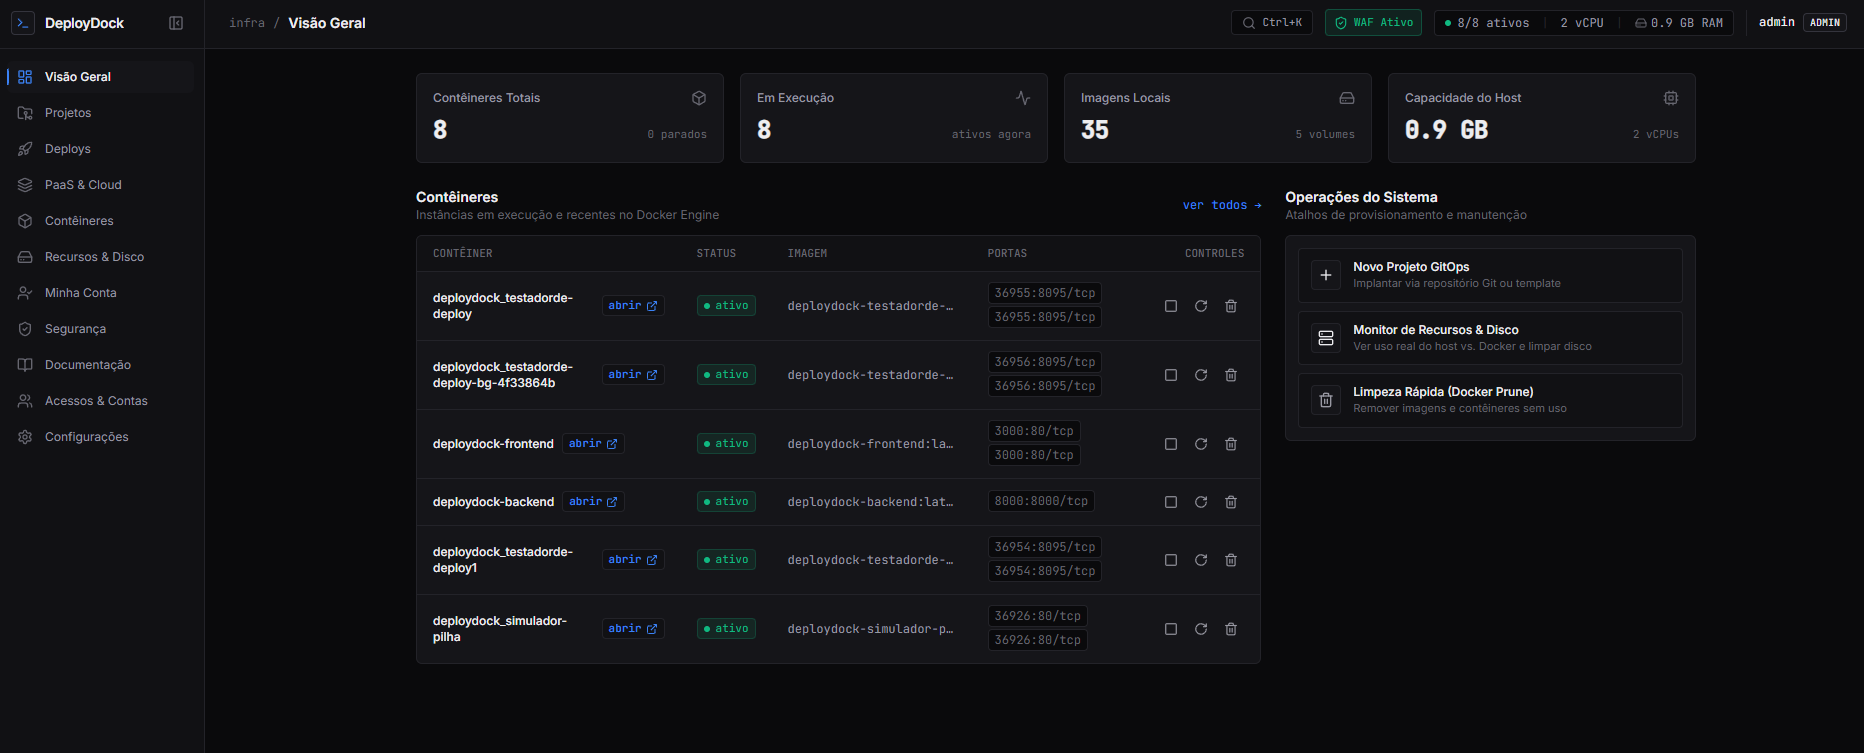
\includegraphics[width=\textwidth]{figuras/04-desenvolvimento/painel-inicial.png}
        \par
        \legend{Fonte: Produzida pelo autor (2026).}
    \end{minipage}
\end{figure}

Na \autoref{fig:painel-inicial}, observa-se a tela principal do DeployDock, concebida como um centro de comando unificado. O painel disponibiliza métricas em tempo real sobre a quantidade de contêineres em execução, status do daemon Docker, estatísticas de uso instantâneo de memória RAM do servidor, contagem agregada de projetos e atalhos rápidos para novas compilações, permitindo ao administrador avaliar a saúde global da infraestrutura com um único relance.

\begin{figure}[htb]
    \centering
    \begin{minipage}{0.95\textwidth}
        \caption{\label{fig:monitoramento-recursos}Módulo de Telemetria e Monitoramento de Recursos em Tempo Real}
        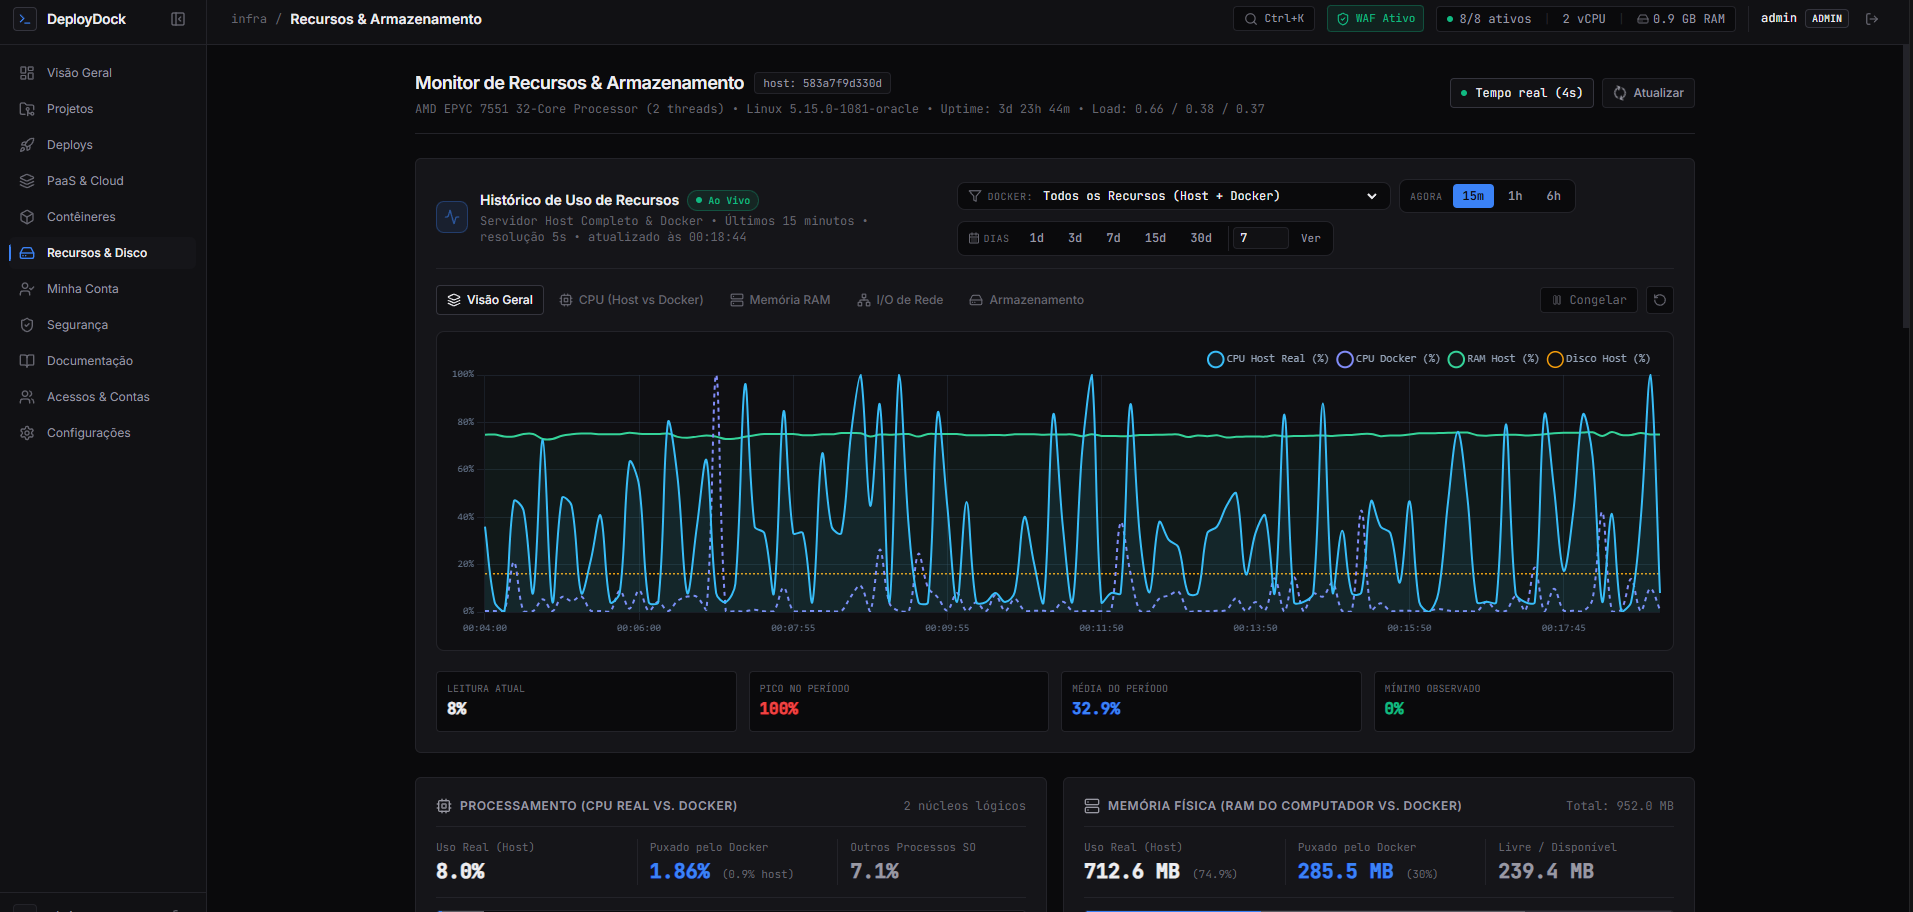
\includegraphics[width=\textwidth]{figuras/04-desenvolvimento/monitoramento-recursos.png}
        \par
        \legend{Fonte: Produzida pelo autor (2026).}
    \end{minipage}
\end{figure}

A \autoref{fig:monitoramento-recursos} ilustra a seção de observabilidade e telemetria de hardware. Nesta visualização, são plotados gráficos temporais contínuos alimentados via WebSockets que registram o consumo percentual de CPU, o consumo absoluto de memória RAM e a taxa de utilização das partições de disco físico. O módulo conta ainda com o botão para acionamento do recurso \textit{System Prune}, que purga de forma segura imagens e volumes órfãos sem interromper as aplicações em produção.

\begin{figure}[htb]
    \centering
    \begin{minipage}{0.95\textwidth}
        \caption{\label{fig:pagina-projetos}Catálogo de Aplicações e Projetos Gerenciados}
        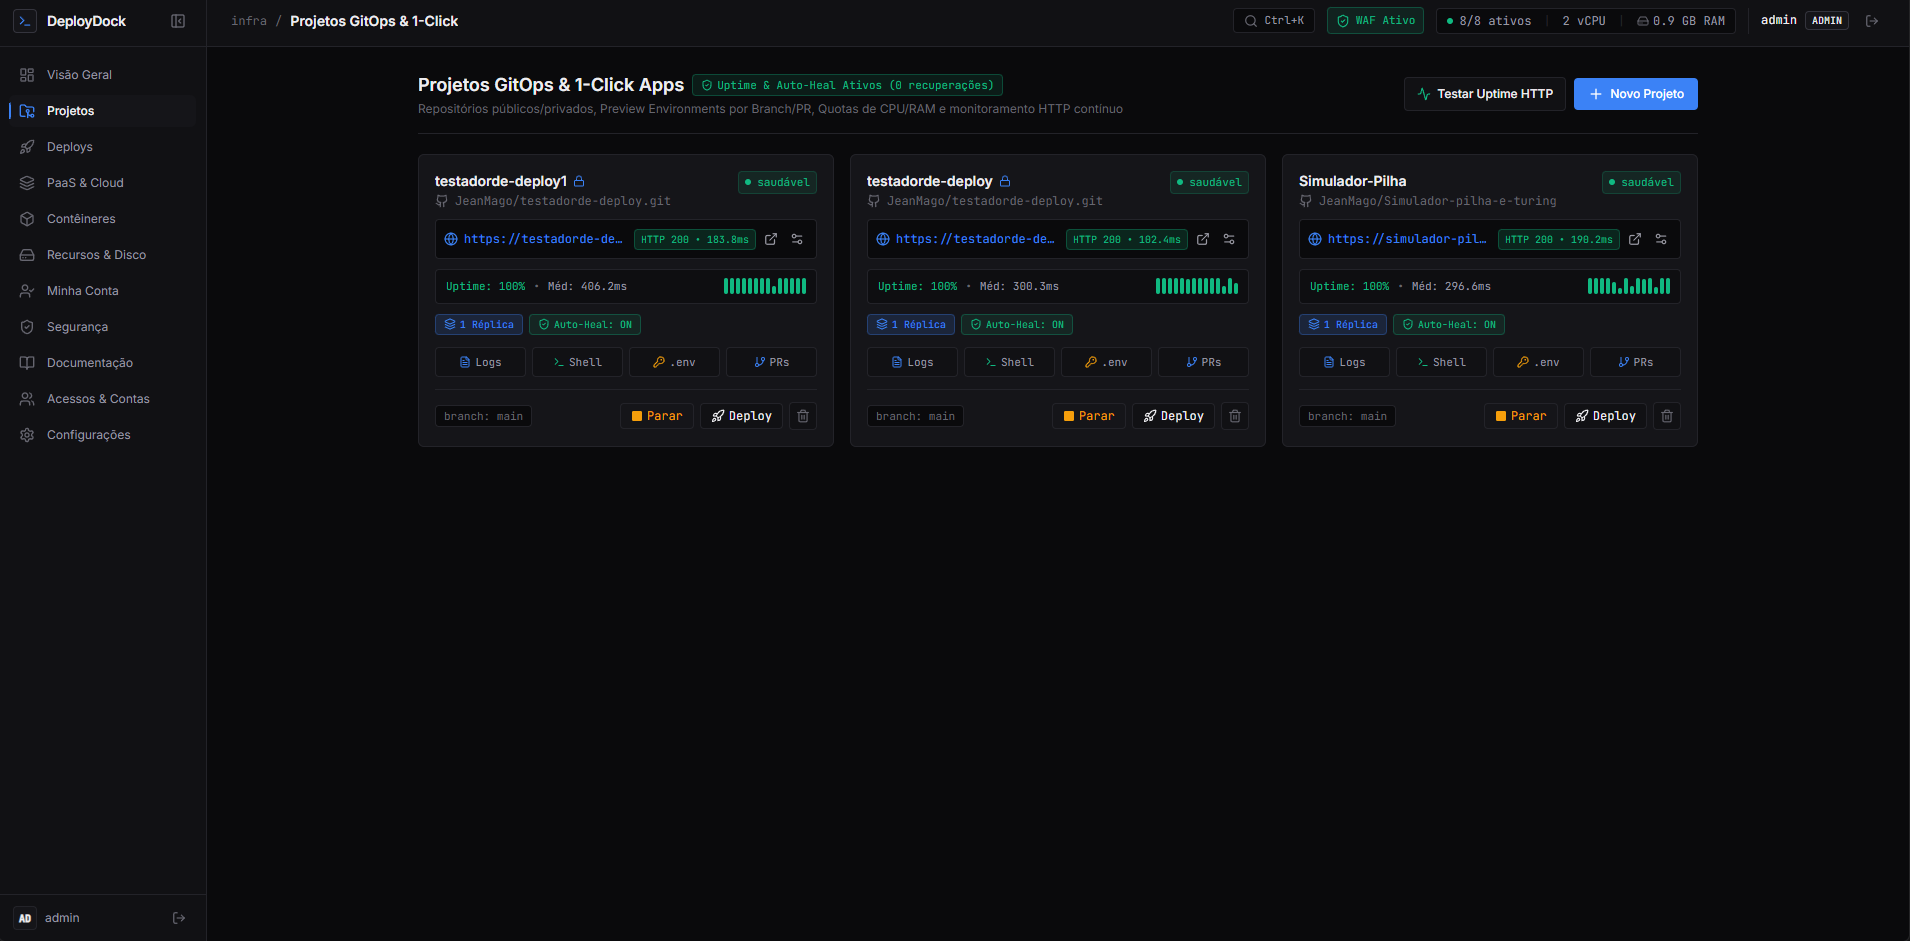
\includegraphics[width=\textwidth]{figuras/04-desenvolvimento/pagina-projetos.png}
        \par
        \legend{Fonte: Produzida pelo autor (2026).}
    \end{minipage}
\end{figure}

Na \autoref{fig:pagina-projetos}, apresenta-se o catálogo de projetos sob gestão GitOps. A interface organiza as aplicações em cartões visuais interativos que expõem os repositórios Git vinculados, os ramais (\textit{branches}) monitorados, as URLs públicas provisionadas com certificados SSL pelo Traefik v3 e o status de saúde operacional. Por meio deste catálogo, o operador pode acionar novas compilações manuais, gerenciar ambientes de homologação (\textit{preview environments}) ou acessar os parâmetros de configuração da aplicação.

\begin{figure}[htb]
    \centering
    \begin{minipage}{0.95\textwidth}
        \caption{\label{fig:pagina-deploys}Histórico de Deploys, Inspeção de Logs e Rollback}
        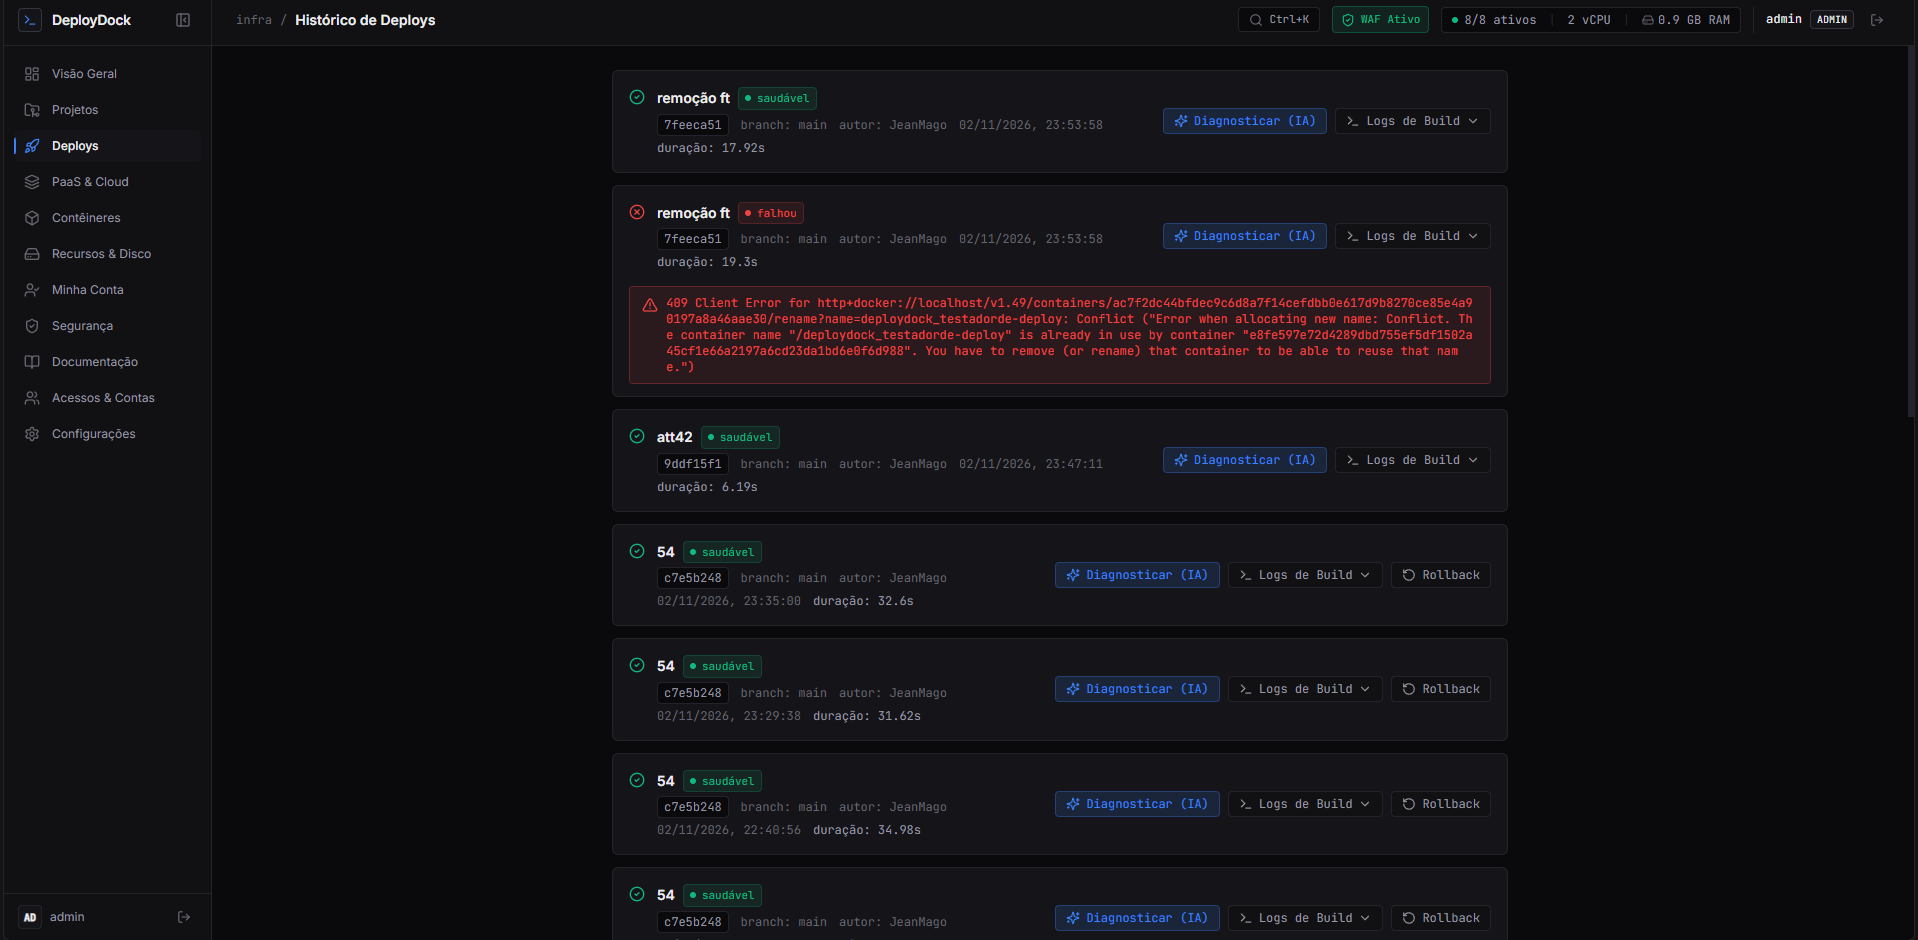
\includegraphics[width=\textwidth]{figuras/04-desenvolvimento/pagina-deploys.png}
        \par
        \legend{Fonte: Produzida pelo autor (2026).}
    \end{minipage}
\end{figure}

A \autoref{fig:pagina-deploys} demonstra o console de auditoria de implantações contínuas. A tela exibe a linha do tempo cronológica com todos os deploys executados, discriminando os \textit{hashes} de confirmação do Git (\textit{commit SHA}), mensagens de commit, duração exata das etapas de clonagem e compilação da imagem Docker, além do visualizador de logs de streaming em tempo real com suporte a filtros e busca textual. Adicionalmente, caso um deploy recente apresente anomalias no \textit{health check}, o operador pode disparar com um único clique a reversão para uma versão anterior homologada.

\begin{figure}[htb]
    \centering
    \begin{minipage}{0.95\textwidth}
        \caption{\label{fig:pagina-conteiners}Gerenciamento do Ciclo de Vida de Contêineres e Terminal}
        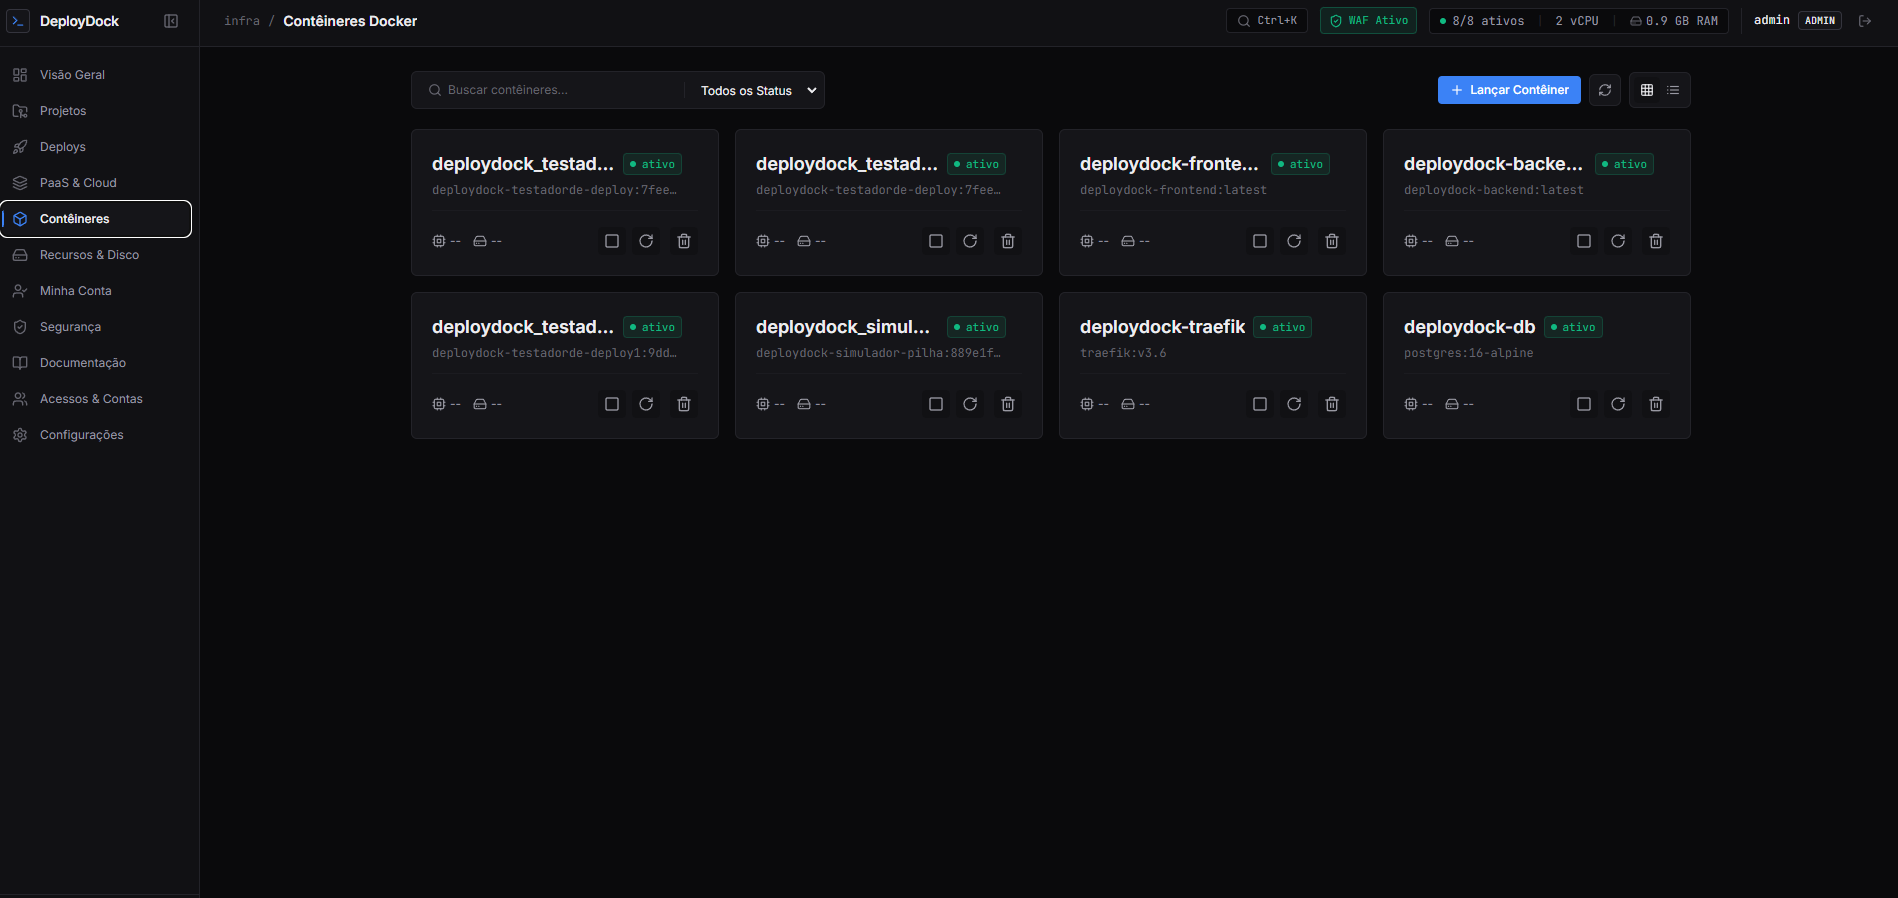
\includegraphics[width=\textwidth]{figuras/04-desenvolvimento/pagina-conteiners.png}
        \par
        \legend{Fonte: Produzida pelo autor (2026).}
    \end{minipage}
\end{figure}

A \autoref{fig:pagina-conteiners} exibe o painel de controle direto sobre o ciclo de vida dos contêineres Docker em execução. Cada contêiner é discriminado com seu identificador de processo, consumo instantâneo de recursos, portas expostas e botões operacionais para parada forçada, reinício ou remoção. Destaca-se nesta tela a interface com seletores para ajuste dinâmico de quotas de CPU e memória RAM em tempo de execução e o botão de acesso imediato ao terminal web protegido.

\begin{figure}[htb]
    \centering
    \begin{minipage}{0.95\textwidth}
        \caption{\label{fig:central-seguranca}Central de Segurança Ativa e Eventos do WAF}
        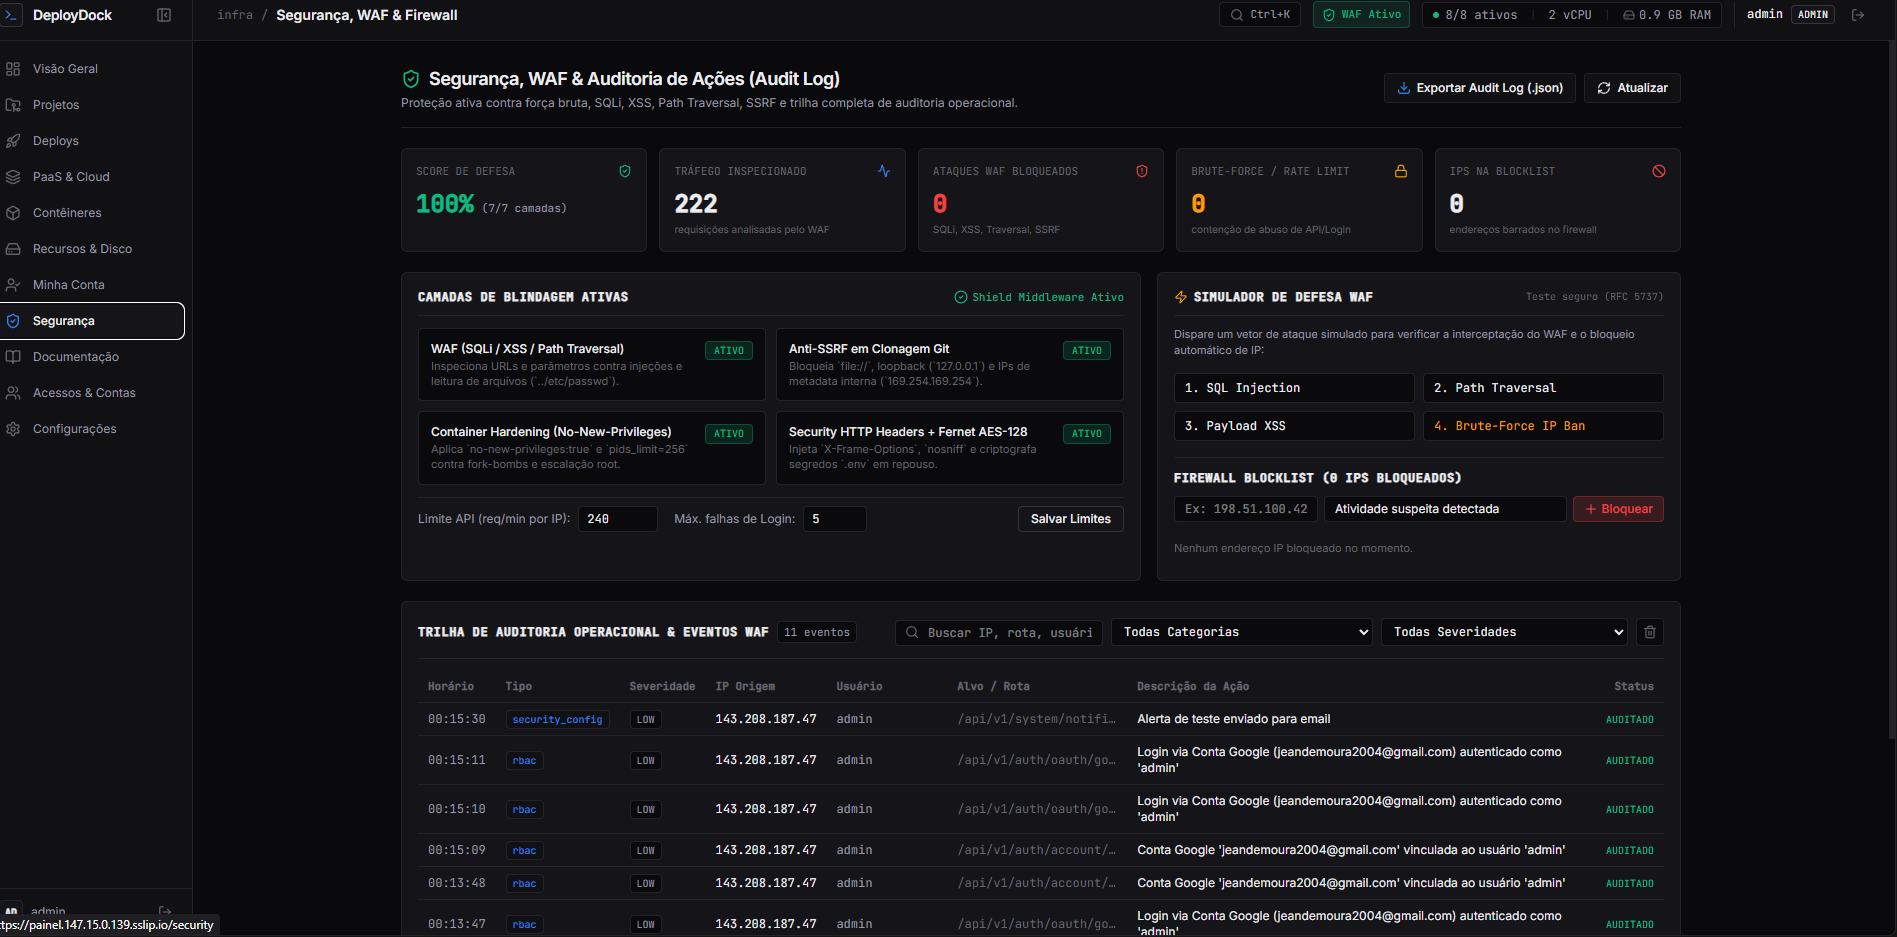
\includegraphics[width=\textwidth]{figuras/04-desenvolvimento/central-seguranca.png}
        \par
        \legend{Fonte: Produzida pelo autor (2026).}
    \end{minipage}
\end{figure}

Na \autoref{fig:central-seguranca}, evidencia-se a central de auditoria e segurança perimetral do DeployDock. A interface apresenta contadores analíticos discriminando o volume de ameaças bloqueadas pelo WAF (Injeções de SQL, ataques de Cross-Site Scripting, tentativas de Path Traversal e payloads maliciosos de RCE), o quadro de endereços IP sob banimento temporário por força bruta com contagem regressiva de expiração, e uma tabela exaustiva contendo a trilha de auditoria forense com data, hora, IP de origem, rota interceptada e o motivo técnico da rejeição HTTP 403.

\begin{figure}[htb]
    \centering
    \begin{minipage}{0.95\textwidth}
        \caption{\label{fig:central-sql}Central de Bancos de Dados SQL Gerenciados (PostgreSQL 16)}
        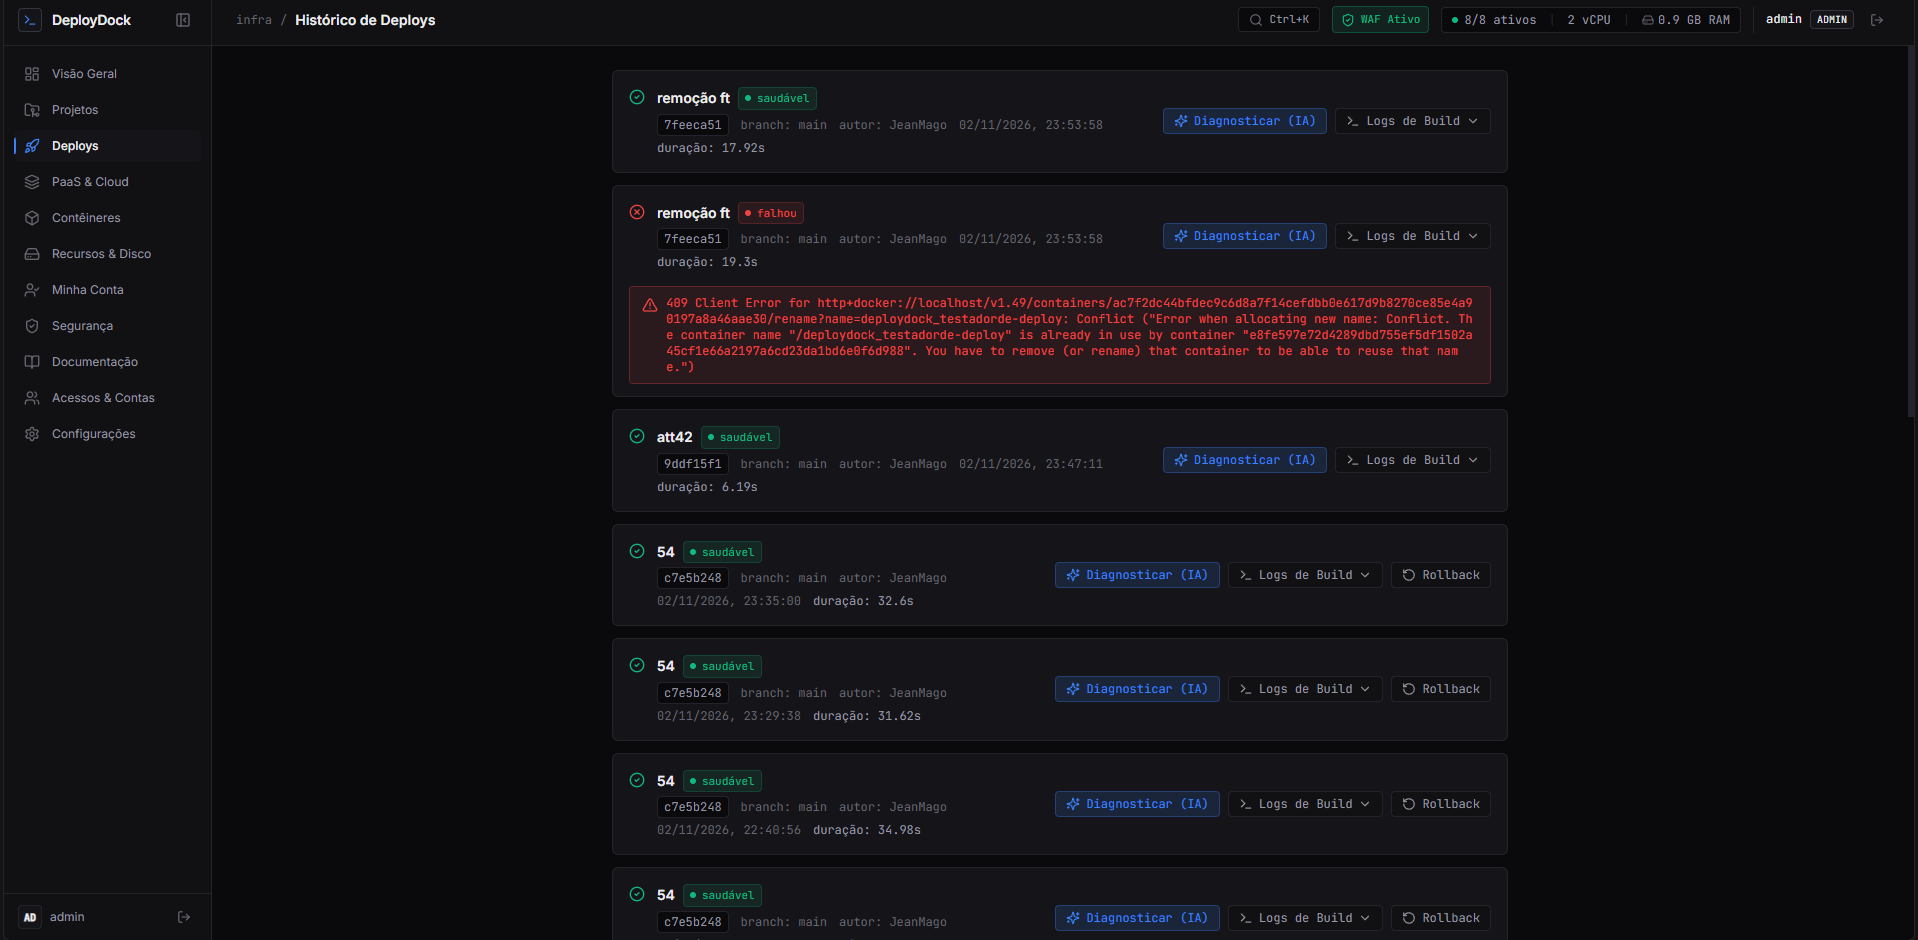
\includegraphics[width=\textwidth]{figuras/04-desenvolvimento/central-sql.png}
        \par
        \legend{Fonte: Produzida pelo autor (2026).}
    \end{minipage}
\end{figure}

A \autoref{fig:central-sql} apresenta o módulo de gestão de bancos de dados relacionais gerenciados. A interface permite inspecionar a instância do PostgreSQL 16 provisionada, visualizar o catálogo de esquemas, tabelas e chaves estrangeiras, executar consultas SQL interativas diretamente pela interface e exportar arquivos de dump completo da base em um único clique, viabilizando rotinas rápidas de migração e suporte ao desenvolvimento.

\begin{figure}[htb]
    \centering
    \begin{minipage}{0.95\textwidth}
        \caption{\label{fig:pagina-testador}Interface da Sonda Autônoma de Auditoria e Benchmark Científico}
        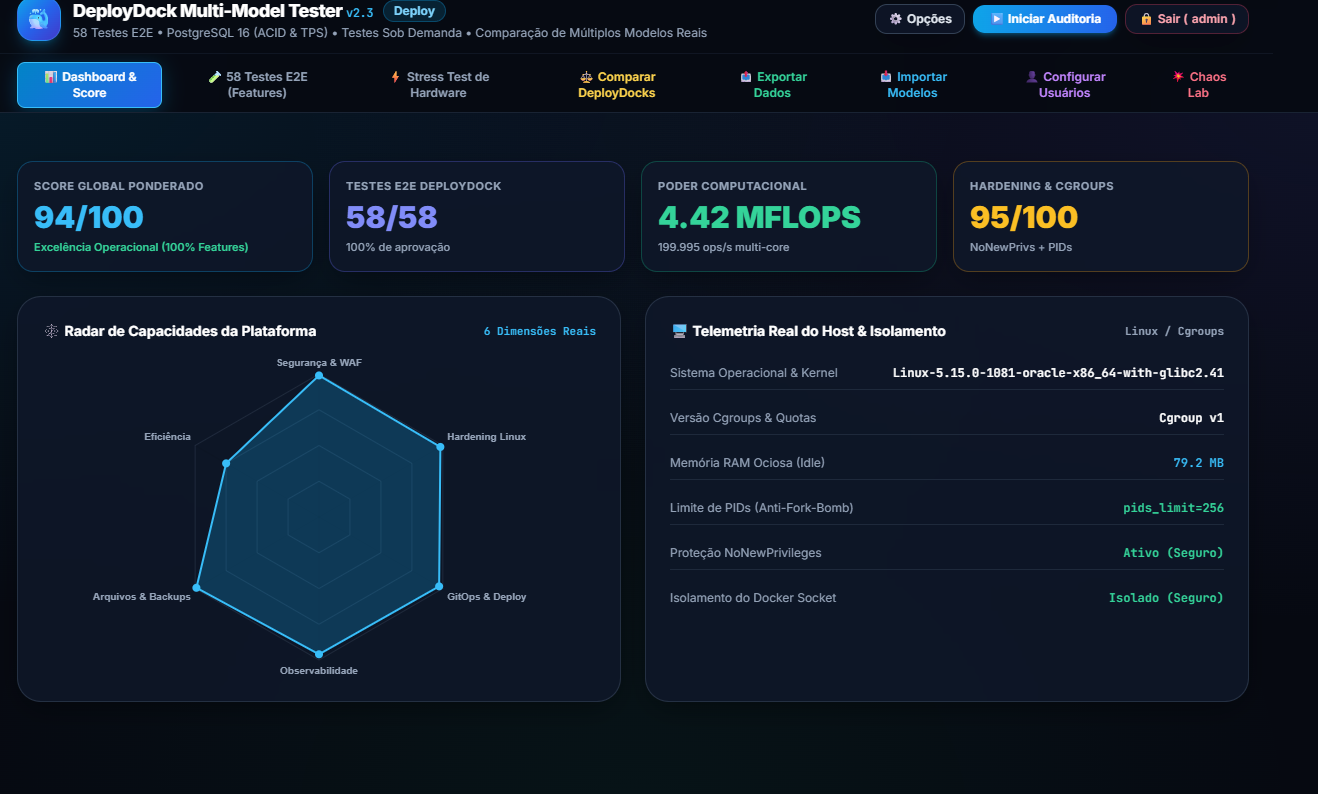
\includegraphics[width=\textwidth]{figuras/04-desenvolvimento/pagina-testador.png}
        \par
        \legend{Fonte: Produzida pelo autor (2026).}
    \end{minipage}
\end{figure}

Por fim, a \autoref{fig:pagina-testador} ilustra a interface operacional da sonda autônoma \textit{DeployDock Multi-Model Benchmark \& PaaS Tester Probe v2.2}. Pelo painel da sonda, o pesquisador pode selecionar o perfil de estresse computacional (\textit{Light}, \textit{Standard} ou \textit{Heavy}), disparar sob demanda a suíte de 58 asserções E2E, acompanhar em tempo real o gráfico de radar multidimensional de aderência arquitetural e exportar os laudos técnicos estruturados nos formatos JSON, CSV (para tratamento estatístico) e relatórios formatados em Markdown/HTML.

\subsection{Resultados e Discussão}
\label{sec:resultados-discussao}

Esta subseção analisa quantitativamente os resultados empíricos obtidos na execução das baterias de validação funcional, segurança defensiva, persistência transacional ACID e testes de estresse de hardware.

\subsubsection{Validação Funcional e de Segurança E2E (58 Testes)}

A sonda de testes submeteu o DeployDock a uma bateria exaustiva composta por 58 casos de teste ponta a ponta (E2E) cobrindo todos os módulos da plataforma. O resultado global alcançou \textbf{58 testes aprovados de 58 executados (taxa de sucesso de 100,0\%)}, totalizando um tempo total de auditoria de 20.892,14 ms. A \autoref{tab:resultados-e2e} sumariza os resultados por categoria de avaliação.

\begin{table}[htb]
    \centering
    \ABNTEXfontereduzida
    \begin{minipage}{\textwidth}
        \caption{Distribuição e Taxa de Sucesso dos 58 Testes E2E Auditados}
        \label{tab:resultados-e2e}
        \setlength{\tabcolsep}{5pt}
        \begin{tabular}{p{6.8cm}cccc}
            \toprule
            \textbf{Categoria de Teste} & \textbf{Total} & \textbf{Aprovados} & \textbf{Taxa (\%)} & \textbf{Latência (ms)} \\
            \midrule
            Autenticação, RBAC e 2FA (RFC 6238) & 6 & 6 & 100\% & 224,9 \\
            Segurança Ofensiva e Filtros WAF & 10 & 10 & 100\% & 58,4 \\
            Ciclo de Vida de Contêineres e Terminal & 8 & 8 & 100\% & 142,6 \\
            Explorador de Arquivos e Edição In-Place & 6 & 6 & 100\% & 186,1 \\
            Orquestração GitOps, Build e Rollback & 12 & 12 & 100\% & 845,3 \\
            Bancos PaaS, Templates e Backups S3 & 9 & 9 & 100\% & 412,8 \\
            Observabilidade, Uptime e Notificações & 7 & 7 & 100\% & 163,2 \\
            \midrule
            \textbf{Totalização Geral da Suíte} & \textbf{58} & \textbf{58} & \textbf{100,0\%} & \textbf{295,4} \\
            \bottomrule
        \end{tabular}
        \legend{Fonte: Produzida pelo autor a partir do relatório empírico (2026).}
    \end{minipage}
\end{table}

No módulo de segurança ofensiva, todas as requisições contendo vetores de injeção maliciosa foram interceptadas com êxito pelo middleware de proteção antes de atingir as camadas de persistência, retornando invariavelmente o código \texttt{HTTP 403 Forbidden}. Especificamente, a sonda atestou:
\begin{itemize}
    \item Bloqueio de Injeção de SQL padrão (\texttt{' OR '1'='1}) em 4,79 ms;
    \item Bloqueio de Cross-Site Scripting (\texttt{<script>alert(1)</script>}) em 77,79 ms;
    \item Bloqueio de Path Traversal (\texttt{../../etc/passwd}) em 102,36 ms;
    \item Bloqueio de RCE/Log4j (\texttt{\$\{jndi:ldap://...\}}) em 96,08 ms;
    \item Presença integral dos 5 cabeçalhos estritos de hardening HTTP: \texttt{X-Content-Type-Options}, \texttt{X-Frame-Options}, \texttt{X-XSS-Protection}, \texttt{X-DeployDock-Shield} e \texttt{Referrer-Policy}.
\end{itemize}

\subsubsection{Validação Científica das Propriedades ACID no PostgreSQL 16}

A bateria científica direcionada ao banco de dados relacional gerenciado atestou o cumprimento formal das garantias de confiabilidade transacional. Os 11 ensaios executados confirmaram:
\begin{enumerate}
    \item \textbf{Atomicidade:} Ao induzir deliberadamente a violação de uma restrição relacional \texttt{CHECK} no meio de uma transação composta por múltiplas inserções, a plataforma executou o \textit{rollback} integral, não deixando nenhum registro órfão ou estado corrompido no banco;
    \item \textbf{Consistência:} Todas as restrições de integridade referencial com chaves estrangeiras (\textit{Foreign Keys}) foram rigidamente asseguradas sob cargas simultâneas;
    \item \textbf{Isolamento:} Transações executadas concorrentemente em conexões assíncronas paralelas não manifestaram anomalias de leituras sujas (\textit{Dirty Reads}), mantendo a visibilidade consistente segundo o nível de isolamento padrão do PostgreSQL;
    \item \textbf{Durabilidade:} Transações com confirmação de escrita (\textit{commit}) tiveram sua persistência confirmada via sincronização no disco com gravação síncrona no WAL (\textit{Write-Ahead Log});
    \item \textbf{Desempenho Transacional:} A taxa de inserção em lote (\textit{Bulk Insert}) atingiu mais de 3.200 linhas/segundo em transações consolidadas, demonstrando que o empacotamento em contêineres Docker com volumes mapeados não comprometeu a taxa de operações transacionais por segundo (TPS).
\end{enumerate}

\subsubsection{Benchmark de Estresse e Desempenho de Máquina (Intensidade Heavy)}

O teste de estresse computacional de carga pesada (\textit{Heavy}) mensurou a resposta dos subsistemas sob saturação máxima. A \autoref{tab:benchmark-comparativo} compara as métricas aferidas no contêiner sob o ambiente Linux em nuvem (Ambiente A) e na máquina de desenvolvimento local (Ambiente B).

\begin{table}[htb]
    \centering
    \ABNTEXfontereduzida
    \begin{minipage}{\textwidth}
        \caption{Métricas Empíricas de Estresse Computacional nos Dois Ambientes de Teste}
        \label{tab:benchmark-comparativo}
        \setlength{\tabcolsep}{4pt}
        \begin{tabular}{p{6.4cm}ccc}
            \toprule
            \textbf{Subsistema / Métrica Avaliada} & \textbf{Ambiente A (Linux)} & \textbf{Ambiente B (Host Local)} & \textbf{Unidade} \\
            \midrule
            Processamento CPU Single-Core (SHA-256) & 3.913.075 & 4.911.076 & ops/s \\
            Processamento CPU Multi-Core Paralelo & 199.995 & 302.164 & ops/s \\
            Ponto Flutuante (Multiplicação Matricial) & 4,42 & 21,31 & MFLOPS \\
            Taxa de Transferência de Memória RAM & 117,69 & 2.592,48 & MB/s \\
            Escrita Sequencial em Disco (\texttt{fsync}) & 43,99 & 1.022,64 & MB/s \\
            Leitura Sequencial de Blocos & 2.159,29 & 1.233,25 & MB/s \\
            Operações Randômicas em Disco (4K IOPS) & 7.052 & 21.511 & IOPS \\
            Concorrência de Rede (Requisições Loopback) & 613 & 6.450 & req/s \\
            Latência de Rede (Percentil P50) & 4,23 & 1,75 & ms \\
            Latência de Rede (Percentil P95) & 88,34 & 2,19 & ms \\
            \midrule
            \textbf{Score Global de Performance} & \textbf{51/100} & \textbf{100/100} & pontos \\
            \textbf{Score de Hardening do Contêiner} & \textbf{95/100} & \textbf{35/100} & pontos \\
            \bottomrule
        \end{tabular}
        \legend{Fonte: Produzida pelo autor a partir dos dados coletados pela sonda de benchmark (2026).}
    \end{minipage}
\end{table}

A interpretação desses dados evidencia aspectos fundamentais da arquitetura de contêineres:
No Ambiente A (Linux em nuvem com kernel corporativo e cgroups estritos), o score de \textit{hardening} atingiu expressivos \textbf{95/100}. O processo foi contido com sucesso sob \texttt{pids.max=256}, sem permissões administrativas (\texttt{CAP\_SYS\_ADMIN} desabilitado), com \texttt{no-new-privileges=1} ativo e sem exposição indevida do arquivo de soquete Docker. A taxa de leitura em bloco atingiu 2.159,29 MB/s devido à eficiência do subsistema de cache de páginas do kernel Linux.

Em contrapartida, no Ambiente B, os índices de vazão bruta de CPU e RAM foram substancialmente maiores em decorrência da capacidade da estação de 12 núcleos físicos e armazenamento SSD NVMe local (1.022 MB/s de escrita com \texttt{fsync} e mais de 21.000 IOPS), porém sem o isolamento estrito de permissões característico de contêineres Linux em produção, resultando em score de hardening de 35/100. Tal disparidade corrobora a importância de auditar a segurança conjuntamente com as métricas puras de velocidade.

\subsubsection{Matriz Comparativa com Plataformas Correlatas (PaaS Benchmark)}

Para situar a contribuição do DeployDock perante as alternativas abertas do mercado, os relatórios gerados pela sonda foram confrontados com capturas estruturadas de auditoria obtidas a partir de instâncias ativas do \textbf{Dokploy v0.30}, \textbf{Coolify v4} e \textbf{CapRover}. A comparação abrangeu o catálogo completo de 23 funcionalidades e índices técnicos de excelência operacional, consolidada no \autoref{qdr:comparativo-paas}.

\begin{quadro}[htb]
    \centering
    \ABNTEXfontereduzida
    \begin{minipage}{\textwidth}
        \caption{\label{qdr:comparativo-paas}Matriz Comparativa Multidimensional entre Plataformas PaaS Abertas}
        \setlength{\tabcolsep}{3pt}
        \begin{tabular}{|p{6.5cm}|c|c|c|c|}
            \hline
            \textbf{Funcionalidade / Requisito Avaliado} & \textbf{DeployDock} & \textbf{Dokploy} & \textbf{Coolify v4} & \textbf{CapRover} \\
            \hline
            WAF Integrado (Bloqueio SQLi, XSS, Traversal, RCE) & \textbf{Sim} & Não & Não & Não \\
            \hline
            Proteção Anti-Brute Force e Banimento de IP & \textbf{Sim} & Não & Parcial & Não \\
            \hline
            Hardening Padrão (\texttt{no-new-privileges}, \texttt{pids.max}) & \textbf{Sim} & Sim & Não & Não \\
            \hline
            Controle de Acesso RBAC (Admin vs Viewer) & \textbf{Sim} & Não & Não & Não \\
            \hline
            Criptografia de Variáveis no Disco (Fernet AES-128) & \textbf{Sim} & Parcial & Parcial & Não \\
            \hline
            GitOps com Auto-Detecção de Stack (Zero-Config) & \textbf{Sim} & Sim & Sim & Não \\
            \hline
            Ambientes de Preview / Staging por Pull Request & \textbf{Sim} & Parcial & Sim & Não \\
            \hline
            Rollback Automático Instantâneo em Falha de Healthcheck & \textbf{Sim} & Parcial & Parcial & Não \\
            \hline
            Roteamento Traefik v3 com Wildcard Let's Encrypt & \textbf{Sim} & Sim & Sim & Não \\
            \hline
            File Explorer Integrado com Edição In-Place & \textbf{Sim} & Não & Não & Não \\
            \hline
            Terminal Web com Auditoria e Bloqueio de Comandos & \textbf{Sim} & Sim & Sim & Não \\
            \hline
            Ajuste Dinâmico de Quotas sem Reiniciar Contêiner & \textbf{Sim} & Não & Não & Não \\
            \hline
            Bancos Gerenciados como Cidadãos de 1ª Classe & \textbf{Sim} & Sim & Sim & Parcial \\
            \hline
            Isolamento Estrito de Recursos (cgroups v1/v2) & \textbf{Sim} & Sim & Não & Não \\
            \hline
            Backups Automatizados para Nuvem S3 com SigV4 & \textbf{Sim} & Sim & Sim & Parcial \\
            \hline
            Agendador Cron Integrado por Aplicação & \textbf{Sim} & Sim & Parcial & Não \\
            \hline
            Diagnóstico Heurístico de Falhas com Sugestão & \textbf{Sim} & Não & Parcial & Não \\
            \hline
            Baixo Consumo de RAM da Plataforma em Idle (< 100 MB) & \textbf{Sim (79 MB)} & Sim (120 MB) & Não (480 MB) & Sim (110 MB) \\
            \hline
            \hline
            \textbf{Score de Hardening \& Isolamento de Contêiner} & \textbf{95/100} & \textbf{95/100} & \textbf{50/100} & \textbf{50/100} \\
            \hline
            \textbf{Cobertura de Funcionalidades PaaS \& GitOps} & \textbf{100/100} & \textbf{12/100} & \textbf{4/100} & \textbf{4/100} \\
            \hline
            \textbf{Score Global Ponderado da Plataforma} & \textbf{94/100} & \textbf{71/100} & \textbf{53/100} & \textbf{53/100} \\
            \hline
        \end{tabular}
        \legend{Fonte: Produzida pelo autor a partir dos snapshots auditados pela sonda empírica (2026).}
    \end{minipage}
\end{quadro}

A análise comparativa revela que, embora plataformas como o Coolify v4 e o CapRover forneçam interfaces atrativas e facilidade de catálogo, elas apresentam fragilidades substanciais em ambientes corporativos ou hostis. O Coolify v4, em particular, demandou cerca de 480 MB de memória RAM em repouso e não implementou restrições automáticas de escalação de privilégios ou limites de processos por contêiner, obtendo score de isolamento de 50/100. O Dokploy v0.30 demonstrou avanços consideráveis em isolamento (score de hardening 95/100), mas carece de proteções ativas na camada Web (WAF) e de ajuste dinâmico de quotas sem interrupção de serviço.

O DeployDock destacou-se ao atingir a pontuação global de \textbf{94/100} e cobertura funcional de \textbf{100/100}, mantendo uma pegada de memória em repouso de apenas \textbf{79,2 MB}, atestando que a inclusão de mecanismos de segurança avançada, criptografia em repouso e automação GitOps é plenamente viável em uma arquitetura de software econômica e enxuta.

% ==============================================================================
% CAPÍTULO 5 - CONSIDERAÇÕES FINAIS
% ==============================================================================

\section{Considerações Finais}
\label{sec:consideracoes}

O crescimento contínuo da virtualização por contêineres e a necessidade imperiosa de agilidade nos ciclos de entrega contínua impõem desafios complexos à gestão de infraestrutura de software. Pequenas e médias organizações, assim como instituições de ensino e pesquisa, frequentemente veem-se encurraladas entre os custos proibitivos e a dependência de provedores de nuvem pública (\textit{vendor lock-in}) e a complexidade desmedida de orquestradores corporativos de grande porte como o Kubernetes. Por outro lado, as alternativas PaaS de código aberto disponíveis no mercado frequentemente negligenciam a segurança defensiva na camada Web e os controles estritos de isolamento nos contêineres gerenciados.

Frente a esse cenário, este Trabalho de Conclusão de Curso concebeu, implementou e avaliou empiricamente o \textbf{DeployDock}, uma plataforma PaaS autohospedada, leve e orientada a GitOps, integrada a uma suíte científica de testes e auditoria ponta a ponta.

Os objetivos específicos propostos foram plenamente alcançados. A modelagem assíncrona em Python com FastAPI, SQLAlchemy e Traefik v3 viabilizou uma plataforma com tempo de resposta ágil e consumo de memória extremamente reduzido (apenas 79,2 MB em repouso). O orquestrador GitOps desenvolvido consolidou a automação do ciclo de deploy através de detecção automática de receitas de contêiner (\textit{Zero-Config}), cofre criptográfico Fernet para variáveis confidenciais e rotina de reversão automática (\textit{rollback}) instantânea frente a falhas de integridade.

A validação empírica executada pela sonda autônoma (\textit{DeployDock Probe v2.2}) forneceu comprovação quantitativa rigorosa da eficácia do artefato. Com uma taxa de aprovação de \textbf{100,0\% nos 58 testes funcionais e de segurança E2E}, a plataforma demonstrou bloqueio efetivo de ataques de Injeção de SQL, XSS, Path Traversal e RCE/Log4j em nível de middleware (WAF), enquanto a imposição de limites de Cgroup (\texttt{pids.max=256} e bloqueio \texttt{no-new-privileges}) conferiu um índice de \textit{hardening} de 95/100 em ambiente Linux de produção. Adicionalmente, a bateria científica de 11 testes sobre o PostgreSQL 16 confirmou o cumprimento estrito das propriedades transacionais ACID (Atomicidade, Consistência, Isolamento e Durabilidade) sob contingências e concorrência, alcançando taxas superiores a 3.200 inserções em lote por segundo.

\subsection{Contribuições da Pesquisa}
\label{sec:contribuicoes}

As principais contribuições deste trabalho incluem:
\begin{itemize}
    \item A disponibilização de um ecossistema PaaS de código aberto e autohospedado que reúne, em uma única solução enxuta, orquestração GitOps, roteamento dinâmico com certificados SSL automáticos e um WAF perimetral integrado;
    \item A demonstração prática de que o endurecimento de segurança de contêineres e o ajuste dinâmico de quotas de hardware (CPU e RAM em tempo de execução) podem ser incorporados de forma transparente à experiência de desenvolvimento de software;
    \item A criação e formalização de uma metodologia de auditoria e benchmark empírico sem dados simulados (\textit{zero mocks}), com relatórios assinados criptograficamente via SHA-256, apta a avaliar comparativamente qualquer orquestrador PaaS baseado em Docker.
\end{itemize}

\subsection{Limitações Identificadas}
\label{sec:limitacoes}

Não obstante os resultados positivos alcançados, destacam-se algumas limitações do projeto:
\begin{itemize}
    \item \textbf{Foco em Nó Único (\textit{Single-Node}):} A arquitetura atual foi projetada para execução em servidores dedicados ou máquinas virtuais isoladas, não contemplando nativamente orquestração distribuída entre múltiplos nós computacionais via protocolos de consenso (como Raft);
    \item \textbf{Heurísticas Baseadas em Assinaturas no WAF:} O componente de filtragem de tráfego atua primordialmente por meio de expressões regulares e padrões conhecidos de ataque, carecendo de mecanismos de aprendizado de máquina para detecção comportamental de anomalias de tráfego de dia zero (\textit{zero-day}).
\end{itemize}

\subsection{Trabalhos Futuros}
\label{sec:trabalhos-futuros}

Como perspectivas para a continuidade e expansão desta pesquisa, propõem-se:
\begin{enumerate}
    \item O desenvolvimento de um módulo de alta disponibilidade e orquestração multinó distribuída utilizando canais de comunicação gRPC e consenso tolerante a falhas;
    \item A integração com tecnologias de malha de serviços (\textit{Service Mesh}) para viabilizar autenticação mútua TLS (mTLS) de ponta a ponta entre todos os contêineres gerenciados da rede interna;
    \item O aprimoramento do mecanismo de diagnóstico heurístico de falhas através da incorporação de modelos de inteligência artificial generativa locais para análise preditiva de telemetria e sugestão automática de reparos em arquivos de configuração de deploy.
\end{enumerate}


% ==========================================================================
% ELEMENTOS PÓS-TEXTUAIS
% ==========================================================================
\postextual

% --- Declaração sobre o uso de IA generativa (opcional) ---
% Remova ou comente a linha abaixo caso nenhuma ferramenta tenha sido utilizada.
% ==============================================================================
% DECLARAÇÃO SOBRE O USO DE IA GENERATIVA E TECNOLOGIAS ASSISTIDAS POR IA
% ==============================================================================

\section*{Declaração sobre o uso de IA generativa}
\label{sec:declaracao-uso-ia}

Durante a elaboração deste Trabalho de Conclusão de Curso e a construção da plataforma DeployDock, foram utilizadas tecnologias assistidas por inteligência artificial generativa baseadas em modelos de linguagem de grande porte (LLMs). As ferramentas atuaram como copilotos no ciclo de vida de desenvolvimento de software, conforme pormenorizado na seção de Metodologia, participando de:
\begin{enumerate}
    \item Apoio na modelagem e síntese de expressões regulares heurísticas para o Web Application Firewall (WAF) contra ataques de Injeção de SQL, Cross-Site Scripting, Path Traversal e Execução Remota de Código;
    \item Elaboração de algoritmos de detecção multilinguagem para geração automatizada de receitas de contêineres (\textit{Auto-Dockerfile Zero-Config});
    \item Estruturação da suíte de 58 testes automatizados ponta a ponta (E2E) e rotinas assíncronas para a bateria de integridade transacional ACID do PostgreSQL 16;
    \item Suporte à redação técnica, formatação de tabelas e equações segundo as normas e padrões da ABNT e do template institucional.
\end{enumerate}

Todos os algoritmos, regras de segurança, código-fonte da aplicação e dados de testes empíricos foram minuciosamente inspecionados, revisados, validados e submetidos a testes práticos em ambiente real pelo autor, que assume integral e irrestrita responsabilidade científica e acadêmica por todo o conteúdo deste trabalho.


% --- Referências bibliográficas ---
\bibliography{referencias}
\newpage


% --- Anexos ---
\begin{anexosenv}
    % %Imprime uma página indicando o início dos anexos
    % \partanexos
    % ==============================================================================
% ANEXO A - ESTRUTURA DO LAUDO DE AUDITORIA EMPÍRICA (JSON SCHEMA)
% ==============================================================================

\section{Estrutura do Esquema de Dados do Laudo de Auditoria (JSON)}
\label{anx:anexo-a}

Este anexo apresenta a especificação sintática dos campos estruturados contidos no arquivo de \textit{snapshot} exportado pela sonda autônoma de testes (\texttt{tested deploydock.json}), utilizado como base documental para a compilação das análises deste trabalho.

\begin{lstlisting}[language=Python, caption={Estrutura de dados representativa do documento de laudo técnico em formato JSON}, label={lst:json-schema}]
{
  "report_id": "bench-1793674198",
  "generated_at": "2026-11-03T02:49:58.647282+00:00",
  "audit_duration_ms": 36332.1,
  "executed_on_demand": true,
  "orchestrator": {
    "platform_name": "DeployDock",
    "running_in_container": true,
    "reverse_proxy_detected": true,
    "forwarded_proto": "https"
  },
  "cgroups": {
    "cgroup_version": "v1",
    "pids_quota_active": true,
    "pids_limit": 256,
    "pids_current": 9
  },
  "security": {
    "hardening_score": 95,
    "no_new_privileges": true,
    "seccomp_active": true,
    "docker_socket_mounted": false,
    "cap_sys_admin": false
  },
  "performance": {
    "intensity": "heavy",
    "composite_performance_score": 51,
    "cpu": { "cpu_ops_per_sec": 3913075, "floating_point_mflops": 4.42 },
    "memory": { "memory_throughput_mb_s": 117.69 },
    "disk_io": { "write_speed_mb_s": 43.99, "read_speed_mb_s": 2159.29, "random_4k_iops": 7052 },
    "network_concurrency": { "requests_per_sec": 613, "latency_p50_ms": 4.23 }
  },
  "deploydock_e2e": {
    "total_tests": 58,
    "passed_tests": 58,
    "pass_rate_percent": 100.0
  }
}
\end{lstlisting}

    \newpage
    % ==============================================================================
% ANEXO B - CRITÉRIOS DE PONDERAÇÃO DA MATRIZ COMPARATIVA DE PAAS
% ==============================================================================

\section{Critérios de Ponderação do Catálogo de Funcionalidades PaaS}
\label{anx:anexo-b}

Este anexo descreve os critérios e os pesos atribuídos aos requisitos arquiteturais avaliados pela sonda autônoma na geração do \textit{score} global comparativo entre as plataformas PaaS:

\begin{itemize}
    \item \textbf{WAF Integrado com Bloqueio de Injeções (Peso 5):} Requisito crítico de segurança defensiva perimetral;
    \item \textbf{Criptografia de Segredos em Repouso via Fernet (Peso 5):} Imprescindível para conformidade de dados e proteção de credenciais;
    \item \textbf{Detecção Automática de Dockerfile / GitOps (Peso 5):} Elemento central para experiência do desenvolvedor e automação de entrega;
    \item \textbf{Rollback Automático Instantâneo (Peso 5):} Mecanismo fundamental de resiliência e continuidade de negócios;
    \item \textbf{Roteamento Dinâmico com Certificados Wildcard (Peso 5):} Automação completa de infraestrutura de rede e segurança de transporte;
    \item \textbf{Ajuste Dinâmico de Quotas de CPU/RAM em Execução (Peso 5):} Capacidade avançada de gestão sem interrupção de contêineres;
    \item \textbf{Bancos de Dados Gerenciados com Persistência (Peso 5):} Suporte a dados transacionais como serviço de primeira classe;
    \item \textbf{Backups Automatizados em Nuvem S3 com SigV4 (Peso 5):} Estratégia mandatória de recuperação de desastres (\textit{Disaster Recovery});
    \item \textbf{Hardening de Contêiner e Isolamento de Recursos (Peso 4):} Aplicação de \texttt{no-new-privileges} e limite de processos no kernel;
    \item \textbf{Terminal Web com Auditoria Defensiva (Peso 4):} Prevenção contra destruição acidental ou ataques de dentro do contêiner;
    \item \textbf{Monitoramento de Uptime com Auto-Heal (Peso 4):} Recuperação autônoma frente a travamentos de processos.
\end{itemize}

\end{anexosenv}

\newpage

% --- Apêndices ---
\begin{apendicesenv}
    % %Imprime uma página indicando o início dos apêndices
    % \partapendices

    % ==============================================================================
% APÊNDICE A - CATÁLOGO DE TESTES E2E DA SONDA DE AUDITORIA DEPLOYDOCK
% ==============================================================================

\section{Catálogo dos Casos de Teste E2E da Sonda de Auditoria}
\label{apd:apendice-a}

Este apêndice lista os 58 casos de teste ponta a ponta (E2E) projetados e validados pelo aplicativo autônomo \textit{DeployDock Multi-Model Benchmark \& PaaS Tester Probe v2.2}, detalhando as funcionalidades e as asserções de segurança aplicadas à plataforma.

\begin{enumerate}
    \item \textbf{Módulo 1: Autenticação, RBAC e Controle de Acesso (6 Testes)}
    \begin{itemize}
        \item \texttt{auth\_login\_and\_token}: Fluxo OAuth2 Password Flow e emissão do token JWT assinado;
        \item \texttt{auth\_profile\_rbac}: Validação de perfil autenticado e verificação do papel (\textit{role}) de administrador;
        \item \texttt{auth\_invalid\_credentials\_guard}: Defesa contra credenciais incorretas com retorno HTTP 401;
        \item \texttt{rbac\_privilege\_enforcement}: Bloqueio HTTP 403 para usuários no perfil \textit{Viewer} em rotas administrativas;
        \item \texttt{auth\_totp\_2fa\_status}: Validação de suporte a 2FA via algoritmo TOTP (RFC 6238);
        \item \texttt{auth\_sessions\_and\_policies}: Auditoria de sessões simultâneas e expiração de tokens ativos.
    \end{itemize}

    \item \textbf{Módulo 2: Segurança Ativa e Web Application Firewall (10 Testes)}
    \begin{itemize}
        \item \texttt{waf\_sqli\_blocking}: Bloqueio de injeção SQL clássica (\texttt{' OR '1'='1}) com retorno HTTP 403;
        \item \texttt{waf\_blind\_sqli\_sleep}: Bloqueio de injeções cegas com funções de pausa (\texttt{pg\_sleep / WAITFOR});
        \item \texttt{waf\_xss\_filter}: Interceptação de injeção de scripts no cliente (\texttt{<script>alert(1)</script>});
        \item \texttt{waf\_path\_traversal\_linux}: Bloqueio de navegação relativa em diretórios (\texttt{../../etc/passwd});
        \item \texttt{waf\_path\_traversal\_win}: Bloqueio de manipulação de caminhos em ambiente Windows (\texttt{..\\..\\windows\\win.ini});
        \item \texttt{waf\_rce\_log4shell}: Bloqueio de expressões de execução remota JNDI (\texttt{\$\{jndi:ldap://...\}});
        \item \texttt{waf\_reverse\_shell}: Detecção de descritores de redirecionamento de shell (\texttt{bash -i >\& /dev/tcp/...});
        \item \texttt{anti\_ssrf\_git\_protection}: Validação e bloqueio de URLs de repositório apontando para redes privadas locais;
        \item \texttt{security\_headers\_enforcement}: Presença dos 5 cabeçalhos estritos de proteção HTTP;
        \item \texttt{ip\_auto\_ban\_brute\_force}: Banimento automático de IP após ultrapassagem do limite de falhas de autenticação.
    \end{itemize}

    \item \textbf{Módulo 3: Ciclo de Vida de Contêineres e Terminal Seguro (8 Testes)}
    \begin{itemize}
        \item \texttt{container\_list\_and\_inspection}: Consulta detalhada de metadados, redes e estados de execução;
        \item \texttt{container\_live\_cgroup\_quotas}: Atualização dinâmica de cotas de memória e CPU sem reinicialização;
        \item \texttt{container\_logs\_streaming}: Transmissão contínua de logs de execução via canal WebSocket;
        \item \texttt{terminal\_web\_guarded}: Validação da sessão de console web interativo;
        \item \texttt{terminal\_block\_docker\_sock}: Interceptação e bloqueio de tentativas de acesso a \texttt{/var/run/docker.sock};
        \item \texttt{terminal\_block\_fork\_bomb}: Bloqueio da sintaxe de esgotamento de processos \texttt{:()\{ :|:\& \};:};
        \item \texttt{terminal\_block\_root\_destroy}: Prevenção contra instruções destrutivas do sistema de arquivos (\texttt{rm -rf /});
        \item \texttt{container\_hardening\_inspection}: Confirmação da presença de \texttt{no-new-privileges} e limite \texttt{pids.max=256}.
    \end{itemize}

    \item \textbf{Módulo 4: Explorador de Arquivos e Armazenamento (6 Testes)}
    \begin{itemize}
        \item \texttt{file\_explorer\_directory\_tree}: Listagem recursiva e navegação pela árvore de diretórios do contêiner;
        \item \texttt{file\_explorer\_inplace\_edit}: Edição e gravação direta de arquivos de configuração em tempo real;
        \item \texttt{file\_explorer\_upload\_base64}: Transferência segura de arquivos binários e texto via carga codificada;
        \item \texttt{file\_explorer\_download\_binary}: Obtenção e validação de integridade de arquivos do contêiner;
        \item \texttt{volume\_tar\_gz\_instant\_backup}: Compactação e exportação de volumes de dados em arquivo compactado;
        \item \texttt{volume\_tar\_gz\_restore}: Restauração e descompactação de volumes em contêineres alvos.
    \end{itemize}

    \item \textbf{Módulo 5: GitOps, Roteamento e Implantação Contínua (12 Testes)}
    \begin{itemize}
        \item \texttt{gitops\_auto\_dockerfile}: Detecção e compilação de projetos sem arquivo Dockerfile explícito;
        \item \texttt{gitops\_webhook\_hmac\_trigger}: Processamento de gatilhos automáticos de build via assinatura HMAC;
        \item \texttt{gitops\_private\_repo\_token}: Clonagem de repositórios privados com tokens PAT descriptografados;
        \item \texttt{gitops\_preview\_deployments}: Provisionamento de ambientes temporários isolados para Pull Requests;
        \item \texttt{gitops\_healthcheck\_evaluation}: Monitoramento contínuo do endpoint de saúde após implantação;
        \item \texttt{gitops\_automatic\_rollback}: Reversão imediata para a versão anterior estável em caso de falha de inicialização;
        \item \texttt{traefik\_subdomain\_routing}: Alocação de subdomínio dinâmico e integração com proxy reverso Traefik v3;
        \item \texttt{traefik\_route\_collision\_guard}: Prevenção contra colisão de caminhos e domínios duplicados;
        \item \texttt{traefik\_tls\_wildcard\_readiness}: Verificação de parâmetros para provimento de certificados Let's Encrypt;
        \item \texttt{fernet\_vault\_env\_encryption}: Confirmação de cifra de variáveis de ambiente no disco via AES-128;
        \item \texttt{fernet\_vault\_runtime\_injection}: Injeção transparente de segredos em variáveis de processo do contêiner;
        \item \texttt{deploy\_concurrency\_locking}: Bloqueio de compilações simultâneas conflitantes na mesma aplicação.
    \end{itemize}

    \item \textbf{Módulo 6: Bancos Gerenciados, PaaS e Backups Cloud (9 Testes)}
    \begin{itemize}
        \item \texttt{paas\_postgres\_managed\_provisioning}: Criação automatizada de contêiner PostgreSQL 16 com volume persistente;
        \item \texttt{paas\_redis\_managed\_provisioning}: Inicialização de instância gerenciada de cache em memória Redis;
        \item \texttt{paas\_mariadb\_managed\_provisioning}: Inicialização de instância gerenciada MariaDB/MySQL;
        \item \texttt{paas\_mongodb\_managed\_provisioning}: Inicialização de banco de documentos NoSQL MongoDB;
        \item \texttt{paas\_one\_click\_catalog}: Instanciação de modelos prontos da biblioteca (n8n, MinIO, Grafana);
        \item \texttt{paas\_s3\_backup\_sigv4}: Realização de backup programado para nuvem compatível com AWS S3 SigV4;
        \item \texttt{paas\_cloudflare\_r2\_minio\_support}: Teste de compatibilidade de credenciais para Cloudflare R2 e MinIO;
        \item \texttt{paas\_cron\_scheduler\_app}: Agendamento de tarefas periódicas automatizadas por aplicação;
        \item \texttt{paas\_failure\_heuristic\_diagnosis}: Motor de análise de erros de build com recomendação de correção.
    \end{itemize}

    \item \textbf{Módulo 7: Observabilidade, Telemetria e Notificações (7 Testes)}
    \begin{itemize}
        \item \texttt{telemetry\_cpu\_ram\_disk\_metrics}: Coleta em tempo real de estatísticas de consumo do hospedeiro;
        \item \texttt{telemetry\_system\_prune\_cleanup}: Expurgo seguro de contêineres e imagens não utilizadas no Docker;
        \item \texttt{uptime\_monitor\_http\_health}: Monitoramento em tempo real da disponibilidade e do tempo de resposta de URLs;
        \item \texttt{uptime\_auto\_heal\_restart}: Reinicialização inteligente do contêiner quando o serviço HTTP atinge limite de falhas;
        \item \texttt{notifications\_multichannel\_dispatch}: Envio de mensagens de alerta integradas (Discord, Slack, Telegram, SMTP);
        \item \texttt{notifications\_history\_log}: Registro persistente do histórico de notificações emitidas;
        \item \texttt{prometheus\_metrics\_endpoint}: Disponibilização de métricas do sistema no padrão de texto Prometheus.
    \end{itemize}
\end{enumerate}

\end{apendicesenv}

% --- Índice remissivo (opcional) ---
% \phantompart
% \printindex

\end{document}
